\documentclass{beamer}
\usepackage{multirow}
\usepackage[utf8]{inputenc}
\usepackage{amsmath}
\usepackage{amssymb}
\usepackage{graphicx}
\usepackage{caption}
\usepackage{subcaption}
\usepackage[table]{xcolor}
\usepackage{algpseudocode}
\usepackage{algorithm}
\usepackage{tikz}
\usetikzlibrary{shapes.geometric, calc, positioning}

\usepackage{Sweave}
\usepackage{float}
\usepackage{hyperref}
\usepackage{comment}
\usepackage[style=authoryear,sorting=ynt, backend=biber]{biblatex}
\setbeamercolor*{bibliography entry title}{fg=black}
\setbeamercolor*{bibliography entry location}{fg=black}
\setbeamercolor*{bibliography entry note}{fg=black}
\setbeamertemplate{bibliography item}{}
\renewcommand*{\bibfont}{\scriptsize}
\addbibresource{../include/reference.bib}

\usepackage{amsmath,amssymb}
\newcommand{\X}{\boldsymbol{X}}
\newcommand{\Y}{\boldsymbol{Y}}
\newcommand{\x}{\boldsymbol{x}}
\renewcommand{\u}{\boldsymbol{u}}
\newcommand{\y}{\boldsymbol{y}}
\newcommand{\z}{\boldsymbol{z}}
\newcommand{\w}{\boldsymbol{w}}
\newcommand{\R}{\boldsymbol{R}}
\newcommand{\Rinv}{\boldsymbol{R}^{-1}}
\renewcommand{\r}{\boldsymbol{r}}
\newcommand{\one}{\mathbf{1}}
\newcommand{\cov}{\textrm{Cov}}
% \usepackage{enumitem}
% \setlistdepth{10}




\usetheme{Madrid}
\usecolortheme{beaver}


\title[]
{Studies in Hyperparameter Tuning, Design Selection and Optimization}
%{Optimizing Uniform Projection Designs: Differential Evolution Tuning, Space-Filling Evaluation, and Kriging-Driven Sequential Optimization}
\subtitle{}

\author[Onyambu, S.] {Samuel Onyambu\\
          Advisor: Hongquan Xu}


\institute[UCLA] % (optional)
{

 Department of Statistics\\
 UCLA

}

\date[]{\today} % (optional)
%{STAT 201B, 10th March 2021}

%\logo{\includegraphics[height=1.5cm]{images/nsf logo.png}}

%End of title page configuration block
%------------------------------------------------------------



%------------------------------------------------------------
%The next block of commands puts the table of contents at the
%beginning of each section and highlights the current section:

\AtBeginSection[]{
 \begin{frame}
   \frametitle{Table of Contents}
   \tableofcontents[currentsection]
\end{frame}
}



\begin{document}

\frame{\titlepage}

\begin{frame}{Table of Contents}
   \tableofcontents
\end{frame}

% \section{Overview of the Presentation}{Main focus areas}
% \begin{itemize}
%   \item optimization
%   \item Differential Evolution
%   \item Uniform Projection Designs (UniPro)
%   \item hyperparameter tuning
% \end{itemize}

\section{Introduction}
\begin{frame}{Introduction}
\begin{itemize}
  \item Optimization algorithms play a pivotal role in tackling complex real-world problems.
  \item Identifying optimal solutions requires efficient exploration of large and often high-dimensional search spaces.
  \item Generation of Optimal Uniform Projection Designs falls under optimization problem
  \item Issues?
  \begin{itemize}
    \item Discrete Search Space
    \item Non-convex Optimization
  \end{itemize}
  \item Methods?
  \begin{itemize}
    \item Modified Differential Evolution
    \item Bayesian Optimization
  \end{itemize}
\end{itemize}
\end{frame}
\begin{frame}{Why DE}
\begin{itemize}
  \item DE has simplistic nature
  \item Strong global search capabilities
  \item Robust performance
  \item Flexibility in a range of applications
  \item High convergence speed for certain problems
  \item parallelizable
\end{itemize}
\end{frame}
\section{Tuning Differential Evolution Algorithm for Constructing Uniform Projection Designs}

\begin{frame}{Why UniPro}
 \begin{itemize}
  \item When only a subset of the input variables are active, uniformity of projected designs in low-dimensional spaces is important.
\item UniPro have good space-filling properties not only in two dimensions, but also in all dimensions. \parencite{sun2019uniform}
\item Uniform projection designs are robust and perform well under other design
criteria eg the maxPro criteria. \parencite{sun2019uniform}
\item No optimal construction method(s) available.
  \end{itemize}
\end{frame}
\begin{frame}{DE Algorithm}
    \begin{itemize}
      \item \textbf{Genetic Representation} Let $\pi_1,\cdots,\pi_N$ be the initial population where each agent $\pi_i = (\pi_{i1},\cdots,\pi_{im})$ is randomly chosen from $\Omega$
      \item \textbf{Mutation} Produce a potential donor.
      $$
      \nu_i = \pi_a + \omega(\pi_b - \pi_c)
      $$
      \item \textbf{Crossover} Blend the current generation of agents with the population potential donors.
      $$
      \mu_{ij}=\begin{cases}
      \nu_{ij} & \text{With probability \textcolor{blue}{pCR} or if } j=j_0\\
      \pi_{ij} & \text{otherwise}
      \end{cases}
      $$
      where $j = 1,\cdots, m$
      \item \textbf{Selection} Adopt the trial agent if it leads to an improvement.
      $$\pi_i = \begin{cases}
          \mu_i&\text{if } h(\mu_i) > h(\pi_i)\\
          \pi_i &\text{otherwise}
      \end{cases}$$
      \item \textbf{Repeat} Repeat steps 2-4 over many generations.
    \end{itemize}
  \end{frame}

  \begin{frame}{DE Algorithm}
    \begin{figure}
    \centering
    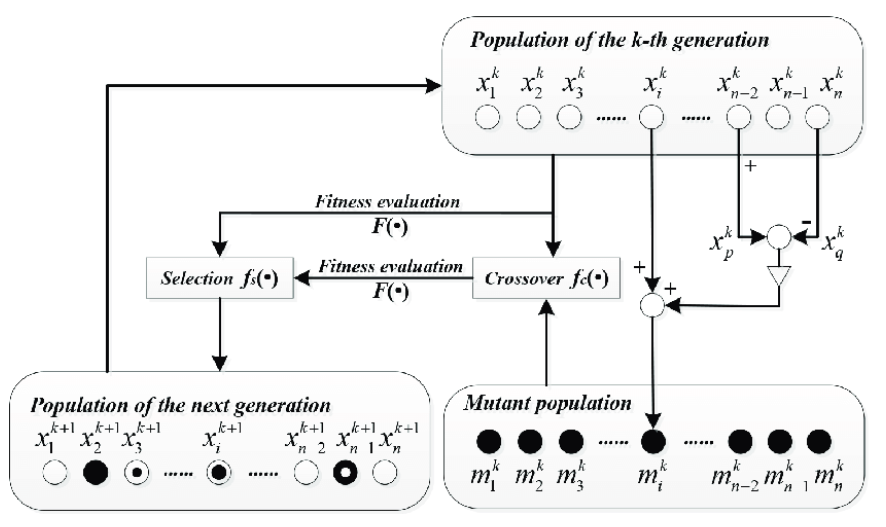
\includegraphics{images/DE.png}
    \caption{outline of DE algorithm}
    \end{figure}
  \end{frame}

  \begin{frame}{Modified DE}
  \begin{itemize}
    \item DE is effective for continuous tasks but needs modification for discrete problems.
    \item \textcite{stokes2023metaheuristic} Proposes modification in the mutation step as:
    \begin{enumerate}
      \item with probability \textcolor{blue}{pGBest}, choose between the global best design and a random design
      \item Generate mutant population by perturbing the columns of the chosen design:\begin{equation}\label{eq:perturbation}
    \nu_i = \operatorname{Perturb}(\pi_a),
    \end{equation}
where
\[
\operatorname{Perturb}(\pi_a): \text{randomly swap 2 elements in }\pi_{aj} \text{ with probability  \textcolor{blue}{pMut}}
\]
\end{enumerate}
\end{itemize}
\end{frame}

\begin{frame}{Modified DE}
Hyperparameters
\begin{itemize}
      \item \textbf{Population Size - $NP$} The size of the population to chose from, with domain chosen as [10, 100].
      \item \textbf{{Itermax}} The maximum number of iterations. Take the values between [500, 1500].
      \item \textbf{Probability of CrossOver - $pCR$} A value between 0.05 and 0.95 that determines whether to use a variable from the $v_i$ or form $\pi_i$.
      \item \textbf{Probability of mutation - $pMut$} A value between 0.05 and 0.95 which determines as to whether a given element in the trial is swapped with another within the same variable.
      \item \textbf{Probability of using global best - $pGBest$} A value between 0.05 and 0.95 that determines whether to use a random agent or the global optimal agent as the trial agent.
    \end{itemize}
\end{frame}


% \begin{frame}

%     The UniPro criterion:

%     $$
%      \phi(D) = \frac{2}{m(m-1)}\sum_{|u| = 2}CD(D_u)
%     $$
%     where $CD$ is the centered $L_2$-discrepancy and defined as:
%     $$
%     \begin{aligned}
% \mathrm{CD}(D)= & \frac{1}{n^2} \sum_{i=1}^n \sum_{j=1}^n \prod_{k=1}^m\left(1+\frac{1}{2}\left|z_{i k}\right|+\frac{1}{2}\left|z_{j k}\right|-\frac{1}{2}\left|z_{i k}-z_{j k}\right|\right) \\
% & -\frac{2}{n} \sum_{i=1}^n \prod_{k=1}^m\left(1+\frac{1}{2}\left|z_{i k}\right|-\frac{1}{2}\left|z_{i k}\right|^2\right)+\left(\frac{13}{12}\right)^m,
% \end{aligned}
% $$
% where $z_{ik} = (2x_{ik} - s+1)/(2s)$\\
% %Fit the second order model, kriging model using matern kernel function and the heterogeneous Gaussian Process to evaluate the designs.
% \end{frame}


\begin{frame}{Objective}
 \begin{itemize}
     \item Objective: Understand the DE hyperparameter surface.
     \item Why? DE performance depends on the hyperparameter settings
     \item How? Tuning the DE hyperparameters Using the UniPro Criterion as the objective function to be minimized.
     \item The UniPro criterion:
     $$
      \phi(D) = \frac{2}{m(m-1)}\sum_{|u| = 2}CD(D_u)
     $$
     where $CD$ is the centered $L_2$-discrepancy and defined as:
     $$
     \begin{aligned}
 \mathrm{CD}(D)= & \frac{1}{n^2} \sum_{i=1}^n \sum_{j=1}^n \prod_{k=1}^m\left(1+\frac{1}{2}\left|z_{i k}\right|+\frac{1}{2}\left|z_{j k}\right|-\frac{1}{2}\left|z_{i k}-z_{j k}\right|\right) \\
 & -\frac{2}{n} \sum_{i=1}^n \prod_{k=1}^m\left(1+\frac{1}{2}\left|z_{i k}\right|-\frac{1}{2}\left|z_{i k}\right|^2\right)+\left(\frac{13}{12}\right)^m,
 \end{aligned}
 $$
 where $z_{ik} = (2x_{ik} - s+1)/(2s)$\\
\end{itemize}
\end{frame}


\begin{frame}{How to Tune}
Issues
\begin{itemize}
  \item Which design to use? ie $\X$
  \item How to collect data? ie $\y$
  \item How do we model the data?
  \item How do we evaluate the data?
\end{itemize}

\resizebox{\textwidth}{!}{
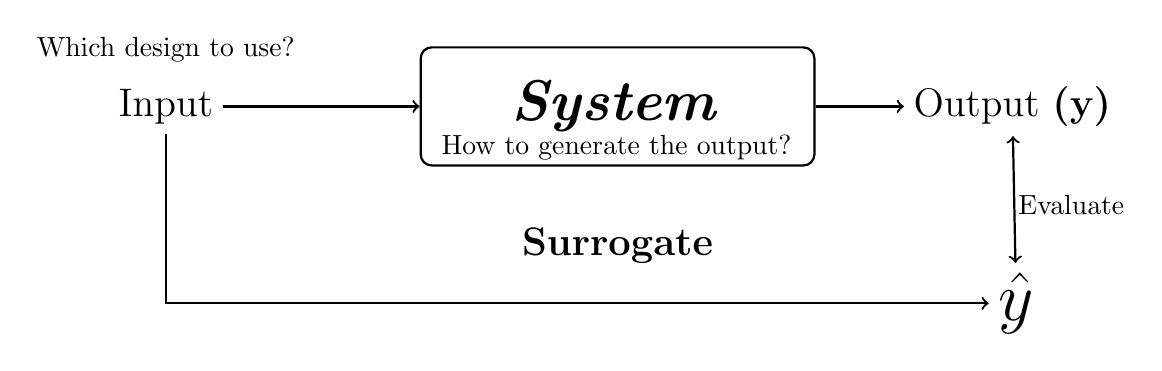
\begin{tikzpicture}[node distance=1.5cm, auto]
    % Rounded rectangle for the population mutation
    \node (input) {\Large{Input}};
    \node[above=0.1cm of input] (x){Which design to use?};
    \node[draw, rounded corners, thick, minimum width=5cm, minimum height=1.5cm, right = 2.5cm of input] (rect1) {};
    % Population label
    \draw[->, thick] (input) -- (rect1);
    \node (system) at ($(rect1.west) + (2.5cm, 0)$) {\huge{\textbf{\textit{System}}}};
    \node[below=-0.2cm of system] {How to generate the output?};
    \node (output) at ($(rect1.east) + (2.5cm, 0)$) {\Large{Output \textbf{(y)}}};
    \draw[->, thick] (rect1) -- (output);
    \node (estimate) at (10.8, -2.5) {\Huge{$\hat{y}$}};
    %\draw[->, thick] (input) --++(0,-2.5) --++(10.8,0) --  (output);
    \draw[->, thick] (input) --++(0,-2.5)--  (estimate);
    \draw[<->, thick] (estimate) --  (output);
    \node at (11.5, -1.25) {Evaluate};
    \node at ($(rect1.south) + (0, -1cm)$){\Large{\textbf{Surrogate}}};
\end{tikzpicture}}
\end{frame}

\begin{frame}{Data Generation}
Obtain $\X$: Use the designs to set the parameters.
  \begin{itemize}
  \item Train Data:
  \begin{itemize}
      \item Factorial Designs -- Physical Experiments
        \begin{itemize}
          \item 43-run Central Composite Design (CCD)
          \item 50-run Orthogonal Array Composite Design (OACD)
        \end{itemize}
      \item Space Filling Designs -- Computer Experiments
      \begin{itemize}
        \item 50-run Latin Hypercube Design (LHD)
        \item 50-run Maximin Distance Design
        \item 50-run Maximum Projection Design (MaxPro)
      \end{itemize}
  \end{itemize}
  \item Test Data:
      \begin{itemize}
        \item $3^5$ \& $4^5$ Full Factorial Design
        \item 243 \& 1024 random Latin Hypercube Design
      \end{itemize}
\end{itemize}

Obtain $\y$: Set the UniPro target size to be considered.
\small{\colorbox{gray!50}{\textcolor{blue!50}{UniPro}(n, m, levels, NP, itermax, pMut, pCR, pGBest, replicates)}}

\end{frame}



\begin{frame}{Modeling and Evaluation}
 \begin{itemize}
   %\item \textbf{Modeling:} %Fit the second order model, kriging model using matern kernel function and the heterogeneous Gaussian Process.
  \item Second order linear model: Mainly for physical experiments\[
\y = \beta_0 + \sum_{i=1}^n \beta_i \x_i + \sum_{i=1}^n \beta_{ii} \x_i^2 + \sum_{i=1}^n \sum_{j=i+1}^n \beta_{ij} \x_i \x_j + \epsilon
\]
  \item Kriging Model: Mainly for computer experiments (deterministic)% An interpolation method used to predict unknown values at specific locations based on known data points.
  $$\y(\x) = f(\x) + Z(\x)$$ where  $f(\x)$ is a deterministic trend and $Z(\x)$ is a GP with mean zero and stationary covariance function $k(\x,\x')$
  \item Heterogeneous Gaussian Process: Computer experiments with error -- need replicates
  $$\y(\x) = f(\x) + Z(\x) + \varepsilon_i$$ where $\varepsilon_i\sim \mathcal{N}(0, r(\x_i))$.
   \item \textbf{Evaluation:} Use RMSE to evaluate the designs.
 \end{itemize}
 \end{frame}

% \iffalse
% \begin{frame}
% \begin{table}
% \caption{\label{tab:tab1}Comparison of designs and model evaluations with target size $30 \times 3$}
% \centering
% \resizebox{\linewidth}{!}{
% \begin{tabular}[t]{|l|r|r|r|r|r|r|r|r|r|r|r|r|}

% \hline
% \multicolumn{1}{|c|}{\textbf{ }} & \multicolumn{6}{|c|}{\textbf{(a) Testing on the $3^5$ FFD}} & \multicolumn{6}{|c|}{\textbf{(b) Testing on the 243 LHD}} \\
% \cline{2-7} \cline{8-13}
% \multicolumn{1}{|c|}{ } & \multicolumn{3}{|c|}{correlation} & \multicolumn{3}{|c|}{RMSE} & \multicolumn{3}{|c|}{correlation} & \multicolumn{3}{|c|}{RMSE} \\
% \cline{2-4} \cline{5-7} \cline{8-10} \cline{11-13}
% Design & lm & km & hetGP & lm & km & hetGP & lm & km & hetGP & lm & km & hetGP\\
% \hline
% ccd3\_43 & 0.88 & 0.88 & 0.88 & 1.51 & 1.59 & 1.62 & 0.65 & 0.03 & 0.60 & 1.62 & 3.75 & 1.51\\
% \hline
% oacd3\_50 & 0.88 & 0.94 & 0.93 & 1.62 & 1.25 & 1.32 & 0.68 & 0.63 & 0.61 & 1.94 & 2.30 & 2.22\\
% \hline
% lhd\_50 & 0.41 & 0.36 & 0.34 & 3.19 & 3.30 & 3.27 & 0.28 & 0.20 & 0.19 & 1.08 & 1.14 & 1.14\\
% \hline
% maximin\_50 & 0.71 & 0.73 & 0.74 & 2.86 & 3.19 & 3.03 & 0.64 & 0.63 & 0.64 & 0.66 & 0.66 & 0.65\\
% \hline
% maxpro\_50 & 0.71 & 0.62 & 0.66 & 2.35 & 2.97 & 2.72 & 0.69 & 0.71 & 0.74 & 0.74 & 0.69 & 0.61\\
% \hline

% \multicolumn{1}{|c|}{\textbf{ }} & \multicolumn{6}{|c|}{\textbf{(c) Testing on the $3^5$ FFD+243 LHD}} & \multicolumn{6}{|c|}{\textbf{(d) Testing on the $4^5$ FFD}} \\
% \cline{2-7} \cline{8-13}
% \multicolumn{1}{|c|}{ } & \multicolumn{3}{|c|}{correlation} & \multicolumn{3}{|c|}{RMSE} & \multicolumn{3}{|c|}{correlation} & \multicolumn{3}{|c|}{RMSE} \\
% \cline{2-4} \cline{5-7} \cline{8-10} \cline{11-13}
% Design & lm & km & hetGP & lm & km & hetGP & lm & km & hetGP & lm & km & hetGP\\
% \hline
% ccd3\_43 & 0.84 & 0.60 & 0.83 & 1.57 & 2.88 & 1.57 & 0.84 & 0.66 & 0.85 & 1.55 & 2.83 & 1.50\\
% \hline
% oacd3\_50 & 0.82 & 0.83 & 0.83 & 1.79 & 1.85 & 1.83 & 0.85 & 0.87 & 0.87 & 1.68 & 1.68 & 1.68\\
% \hline
% lhd\_50 & 0.42 & 0.35 & 0.36 & 2.38 & 2.47 & 2.45 & 0.45 & 0.39 & 0.37 & 2.47 & 2.57 & 2.56\\
% \hline
% maximin\_50 & 0.69 & 0.63 & 0.68 & 2.08 & 2.31 & 2.19 & 0.74 & 0.75 & 0.76 & 2.16 & 2.38 & 2.27\\
% \hline
% maxpro\_50 & 0.74 & 0.60 & 0.68 & 1.75 & 2.15 & 1.98 & 0.74 & 0.67 & 0.71 & 1.80 & 2.22 & 2.03\\
% \hline
% \end{tabular}}
% \end{table}
% \end{frame}
% \fi




% \begin{frame}
% \begin{itemize}
%   \item Second order linear model: \[
% \y = \beta_0 + \sum_{i=1}^n \beta_i \x_i + \sum_{i=1}^n \beta_{ii} \x_i^2 + \sum_{i=1}^n \sum_{j=i+1}^n \beta_{ij} \x_i \x_j + \epsilon
% \]
%   \item Kriging Model: An interpolation method used to predict unknown values at specific locations based on known data points.
%   $$\y(\x) = f(\x) + Z(\x)$$ where  $f(\x)$ is a deterministic trend and $Z(\x)$ is a GP with mean zero and stationary covariance function $k(\x,\x')$
%   \item Heterogeneous Gaussian Process:
%   $$\y(\x) = f(\x) + Z(\x) + \varepsilon_i$$ where $\varepsilon_i\sim \mathcal{N}(0, r(\x_i))$.
% \end{itemize}
% \end{frame}



\begin{frame}
\begin{figure}%[!ht]
\centering
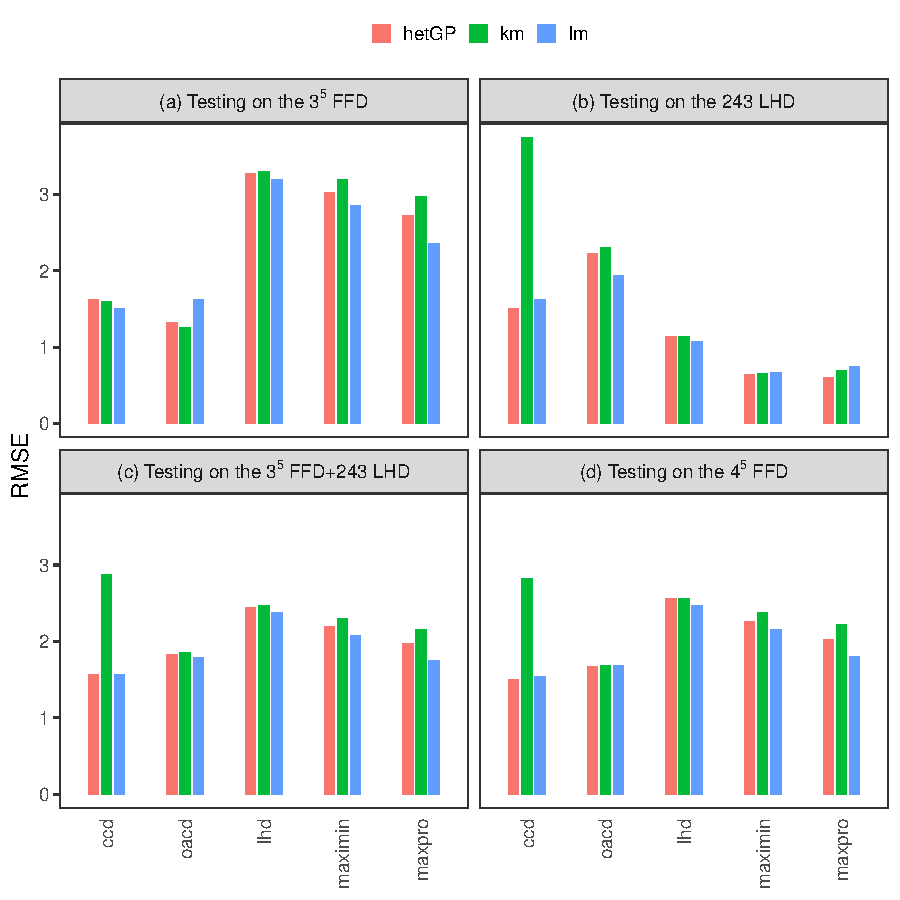
\includegraphics[height=7cm]{../chapters/DE/pdfs/barplots1}
\caption{Comparison of RMSE with target size $30\times3$}
\label{barplots1}
\end{figure}
\end{frame}


% \iffalse
% \begin{frame}
% \scriptsize
% \begin{table}
% \caption{\label{tab:tab3}Comparison of designs and model evaluations with target size $70 \times 7$}
% \centering
% \resizebox{\linewidth}{!}{
% \begin{tabular}[t]{|l|r|r|r|r|r|r|r|r|r|r|r|r|}
% \hline
% \multicolumn{1}{|c|}{\textbf{ }} & \multicolumn{6}{|c|}{\textbf{(a) Testing on the $3^5$ FFD}} & \multicolumn{6}{|c|}{\textbf{(b) Testing on the 243 LHD}} \\
% \cline{2-7} \cline{8-13}
% \multicolumn{1}{|c|}{ } & \multicolumn{3}{|c|}{correlation} & \multicolumn{3}{|c|}{RMSE} & \multicolumn{3}{|c|}{correlation} & \multicolumn{3}{|c|}{RMSE} \\
% \cline{2-4} \cline{5-7} \cline{8-10} \cline{11-13}
% Design & lm & km & hetGP & lm & km & hetGP & lm & km & hetGP & lm & km & hetGP\\
% \hline
% ccd3\_43 & 0.93 & 0.96 & 0.94 & 1.25 & 1.01 & 1.18 & 0.81 & 0.84 & 0.83 & 1.46 & 1.82 & 1.84\\
% \hline
% oacd3\_50 & 0.94 & 0.97 & 0.97 & 1.22 & 0.91 & 0.86 & 0.83 & 0.88 & 0.92 & 1.39 & 1.54 & 1.18\\
% \hline
% lhd\_50 & 0.83 & 0.84 & 0.82 & 2.15 & 2.28 & 2.18 & 0.94 & 0.95 & 0.95 & 0.75 & 0.69 & 0.72\\
% \hline
% maximin\_50 & 0.87 & 0.87 & 0.81 & 1.77 & 2.09 & 2.14 & 0.94 & 0.94 & 0.93 & 0.82 & 0.80 & 0.86\\
% \hline
% maxpro\_50 & 0.88 & 0.88 & 0.87 & 1.80 & 2.01 & 1.89 & 0.94 & 0.95 & 0.95 & 0.80 & 0.71 & 0.70\\
% \hline
% \multicolumn{1}{|c|}{\textbf{ }} & \multicolumn{6}{|c|}{\textbf{(c) Testing on the $3^5$ FFD+243 LHD}} & \multicolumn{6}{|c|}{\textbf{(d) Testing on the $4^5$ FFD}} \\
% \cline{2-7} \cline{8-13}
% \multicolumn{1}{|c|}{ } & \multicolumn{3}{|c|}{correlation} & \multicolumn{3}{|c|}{RMSE} & \multicolumn{3}{|c|}{correlation} & \multicolumn{3}{|c|}{RMSE} \\
% \cline{2-4} \cline{5-7} \cline{8-10} \cline{11-13}
% Design & lm & km & hetGP & lm & km & hetGP & lm & km & hetGP & lm & km & hetGP\\
% \hline
% ccd3\_43 & 0.90 & 0.91 & 0.90 & 1.36 & 1.47 & 1.54 & 0.92 & 0.94 & 0.93 & 1.28 & 1.26 & 1.33\\
% \hline
% oacd3\_50 & 0.91 & 0.93 & 0.95 & 1.30 & 1.27 & 1.03 & 0.92 & 0.94 & 0.95 & 1.29 & 1.21 & 1.06\\
% \hline
% lhd\_50 & 0.87 & 0.87 & 0.87 & 1.61 & 1.69 & 1.62 & 0.86 & 0.87 & 0.86 & 1.81 & 1.85 & 1.79\\
% \hline
% maximin\_50 & 0.90 & 0.88 & 0.86 & 1.38 & 1.58 & 1.63 & 0.89 & 0.89 & 0.86 & 1.49 & 1.67 & 1.75\\
% \hline
% maxpro\_50 & 0.90 & 0.89 & 0.90 & 1.39 & 1.51 & 1.43 & 0.90 & 0.90 & 0.90 & 1.49 & 1.58 & 1.51\\
% \hline
% \end{tabular} }
% \end{table}
% \end{frame}
% \fi

\begin{frame}

\begin{figure}%[!ht]
\centering
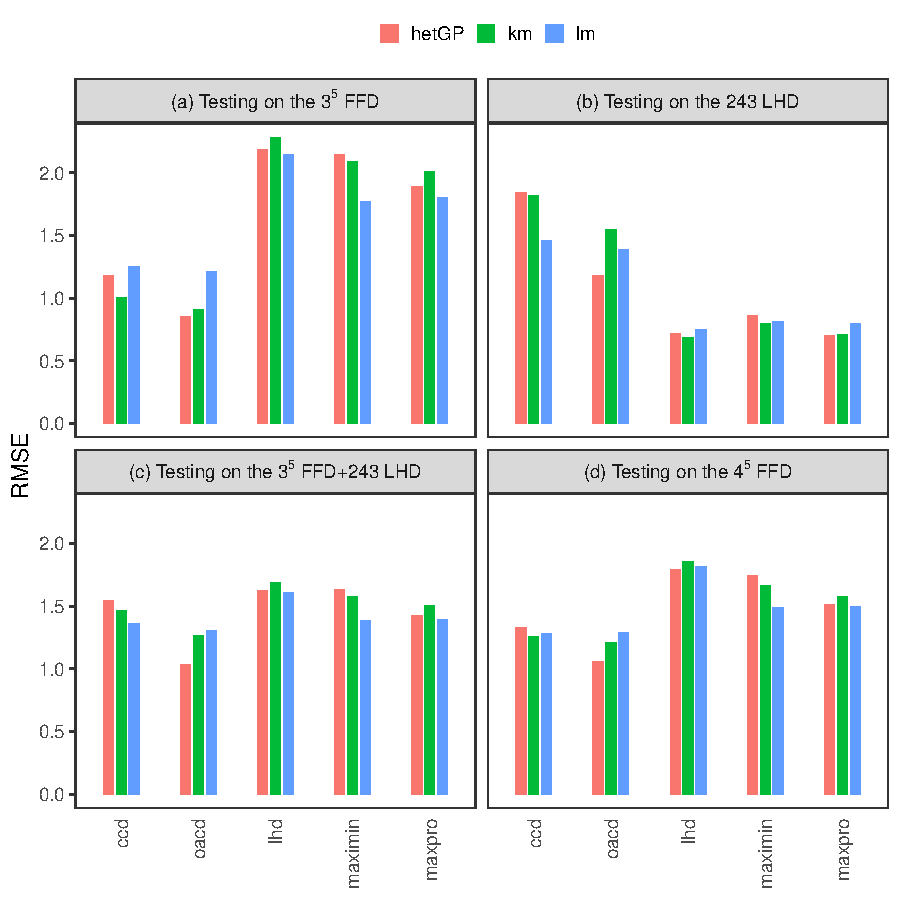
\includegraphics[height=7cm]{../chapters/DE/pdfs/barplots3}
\caption{Comparison of RMSE with target size $70\times7$}
\label{barplots3}
\end{figure}
\end{frame}
\begin{frame}{Results}
\begin{itemize}
\item The performance of the training data set depends on the nature of the testing data set.
\item The composite designs, CCD and OACD, seem to be better when tested on the $3^5$ FFD.
\item The space filling designs (random LHD, maximin LHD, and maxpro LHD) did better when tested on the 243-run random LHD.
\item OACD robust over CCD.
\item Thus: Use OACD for hyperparameter initialization.
\item Models?  There seems to be no striking observation to be made as to whether one fitting method performs better than the other two, with  exception for one $30 \times 3$ case when the kriging model fitting to the CCD training data had a much higher RMSE value than the other cases.
\end{itemize}
\end{frame}

\begin{frame}{Factor Importance}
\scriptsize
\begin{table}
\begin{center}
\renewcommand{\arraystretch}{0.5}
\resizebox{\linewidth}{!}{
\begin{tabular}{l c c c c}
\hline
 & ccd3\_43 & oacd3\_50 & maximin\_50 & maxpro\_50 \\
\hline
(Intercept)    & $0.3815^{***}$  & $0.3876^{***}$  & $0.3878^{***}$  & $0.3814^{***}$  \\
\rowcolor{green!50}
NP             & $-0.0134^{***}$ & $-0.0143^{***}$ & $-0.0042^{***}$ & $-0.0055^{*}$   \\
pMut           & $0.0020$        & $0.0028$        & $0.0043^{***}$  & $0.0045^{*}$    \\
\rowcolor{blue!50}
pGBest         & $-0.0204^{***}$ & $-0.0224^{***}$ & $-0.0047^{***}$ & $-0.0082^{***}$ \\
pCR            & $-0.0022$       & $-0.0030$       & $0.0004$        & $0.0007$        \\
\rowcolor{red!50}
itermax        & $-0.0146^{***}$ & $-0.0152^{***}$ & $-0.0046^{***}$ & $-0.0021$       \\
itermax\_q     & $0.0090$        & $-0.0081$       & $0.0011$        & $0.0057$        \\
NP\_q          & $0.0119$        & $0.0080$        & $0.0022$        & $-0.0004$       \\
pCR\_q         & $0.0071$        & $0.0074$        & $-0.0008$       & $0.0049$        \\
pGBest\_q      & $0.0083$        & $0.0192^{*}$    & $0.0035$        & $0.0159^{***}$  \\
pMut\_q        & $0.0150$        & $0.0174^{*}$    & $0.0083^{***}$  & $0.0104^{*}$    \\
NP:pMut        & $0.0058$        & $0.0064^{*}$    & $-0.0002$       & $-0.0037$       \\
NP:pGBest      & $-0.0041$       & $-0.0038$       & $0.0017$        & $0.0006$        \\
NP:pCR         & $0.0002$        & $-0.0007$       & $-0.0006$       & $-0.0002$       \\
NP:itermax     & $0.0049$        & $0.0033$        & $0.0023$        & $0.0052$        \\
pMut:pGBest    & $-0.0080^{*}$   & $-0.0093^{***}$ & $-0.0089^{***}$ & $-0.0139^{**}$  \\
\rowcolor{red!50}
pMut:pCR       & $0.0203^{***}$  & $0.0197^{***}$  & $0.0042^{**}$   & $0.0018$        \\
pMut:itermax   & $0.0032$        & $0.0025$        & $-0.0061^{***}$ & $0.0004$        \\
pGBest:pCR     & $0.0034$        & $0.0036$        & $0.0000$        & $0.0051$        \\
pGBest:itermax & $0.0057$        & $0.0068^{**}$   & $0.0076^{***}$  & $0.0058$        \\
pCR:itermax    & $0.0037$        & $0.0021$        & $0.0018$        & $0.0040$        \\
\hline
R$^2$          & $0.9034$        & $0.9235$        & $0.8970$        & $0.7297$        \\
Adj. R$^2$     & $0.8157$        & \cellcolor{blue!25}$0.8708$        & $0.8260$        & \cellcolor{yellow!50}$0.5433$        \\
Num. obs.      & $43$            & $50$            & $50$            & $50$            \\
\hline
\multicolumn{5}{l}{\scriptsize{$^{***}p<0.001$; $^{**}p<0.01$; $^{*}p<0.05$}}
\end{tabular}}
\caption{Statistical models}
\label{table:coefficients}
\end{center}
\end{table}
\end{frame}

\begin{frame}{Results}
\begin{itemize}
  \item The model obtained from using the maxpro LHD  training data is the worst performing.
  \item Does not capture important main effects.
  \item The model obtained by using OACD performs the best. It has an adjusted $R^2$ of $0.87$. Captures important main effects and interactions.
  \item CCD might be a little worse than OACD because of the fewer number of points $(43)$ used for training compared to the other models which used $50$ points.
  \item The model from the CCD does not identify any of the quadratic effects to be significant while the other modes do.
  \item The main effects of three hyperparameters (NP, itermax and pGBest) are very significant. Should be set at the maximum level
\end{itemize}
\end{frame}

% \begin{frame}
% \begin{figure}{Interaction with pMut}
% \centering
% 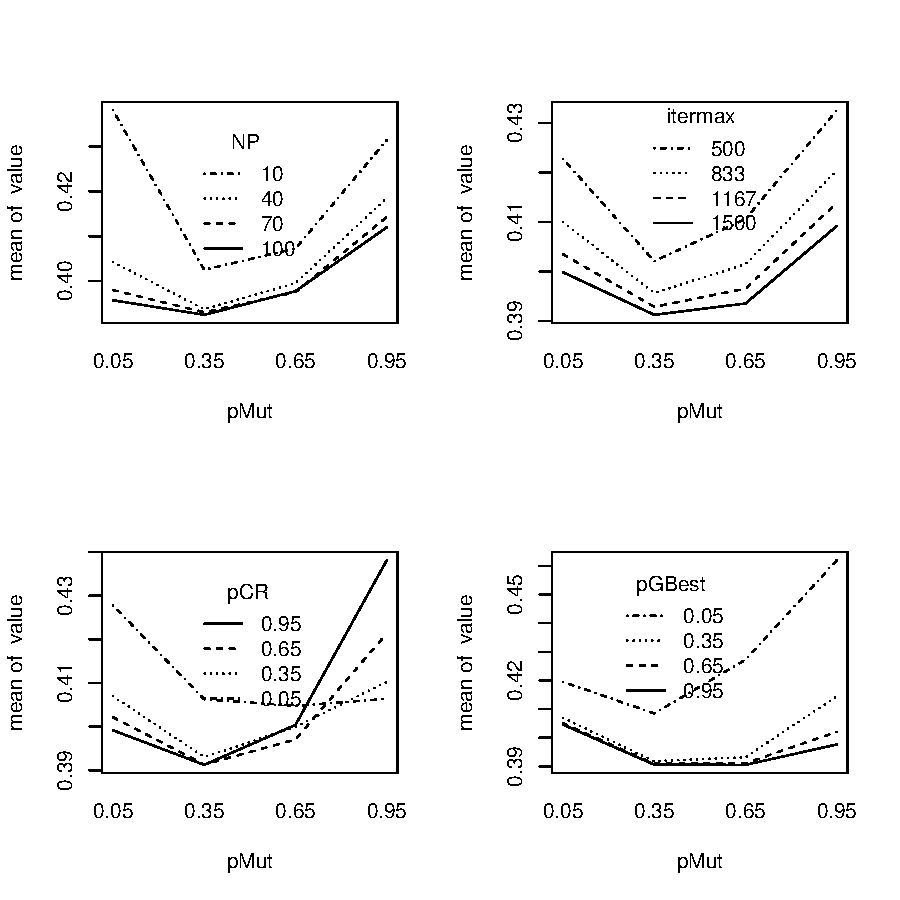
\includegraphics[scale=0.5]{../chapters/DE/pdfs/interactions}
% \caption{Interaction plots involving pMut based on the $4^5$ FFD and target size $30\times3$.}
% \label{interaction}
% \end{figure}
% \end{frame}

\begin{frame}
\begin{figure}{Contours}
\centering
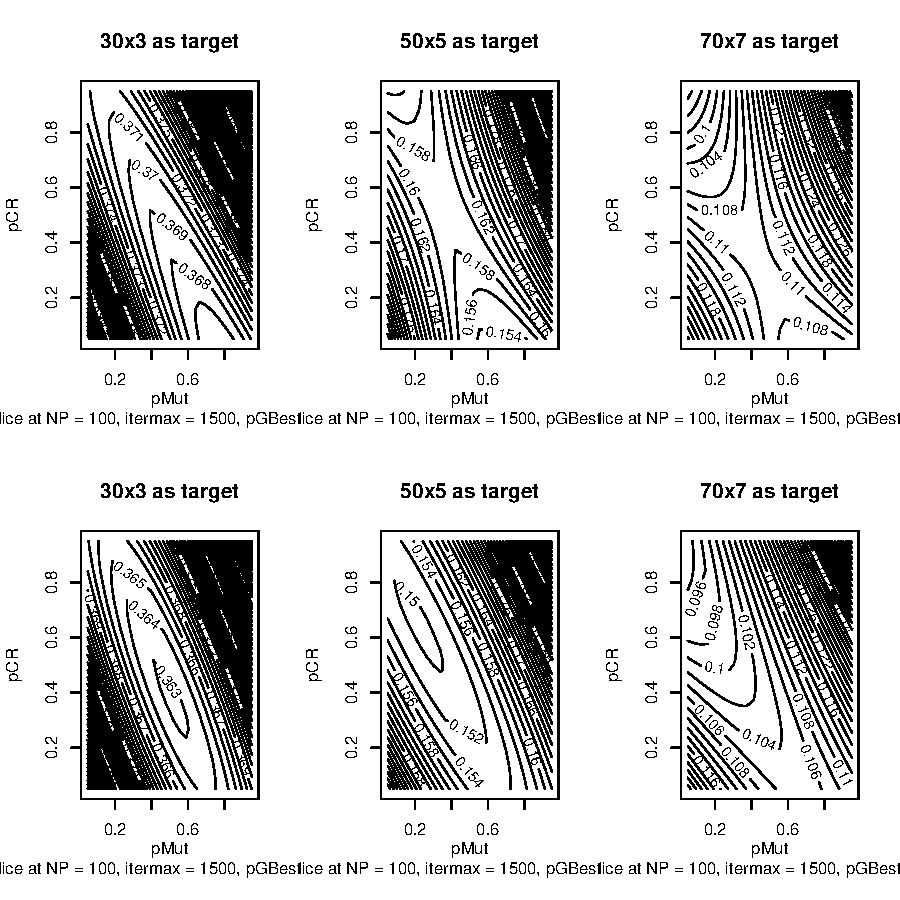
\includegraphics[height=7cm width=15cm]{../chapters/DE/pdfs/contours}
\caption{Contour plots of pMut and pCR while fixing other hyperparameters at high levels. Top row uses CCD as the training data; bottom row uses OACD as training data.}
\label{fig:contours}
\end{figure}
\end{frame}


% \begin{frame}{Optimal Settings}
% \begin{itemize}
%   \item NP -- 100
%   \item Itermax -- 1500
%   \item pGBest -- 0.95
%   \item pMut
%   \begin{itemize}
%     \item $30\times3$ -- 0.95
%     \item  $50\times5$ -- 0.25
%     \item $70\times7$ -- 0.15
%   \end{itemize}
%   \item pCR
%   \begin{itemize}
%     \item $30\times3$ -- 0.05
%     \item  $50\times5$ -- 0.75
%     \item $70\times7$ -- 0.85
%   \end{itemize}
% \end{itemize}
% \end{frame}

% \begin{frame}{Performance of the DE algorithms under three setttings: DE1, DE4 and DEoptim (optimal settings)}
%    \begin{figure}
%       \centering
%       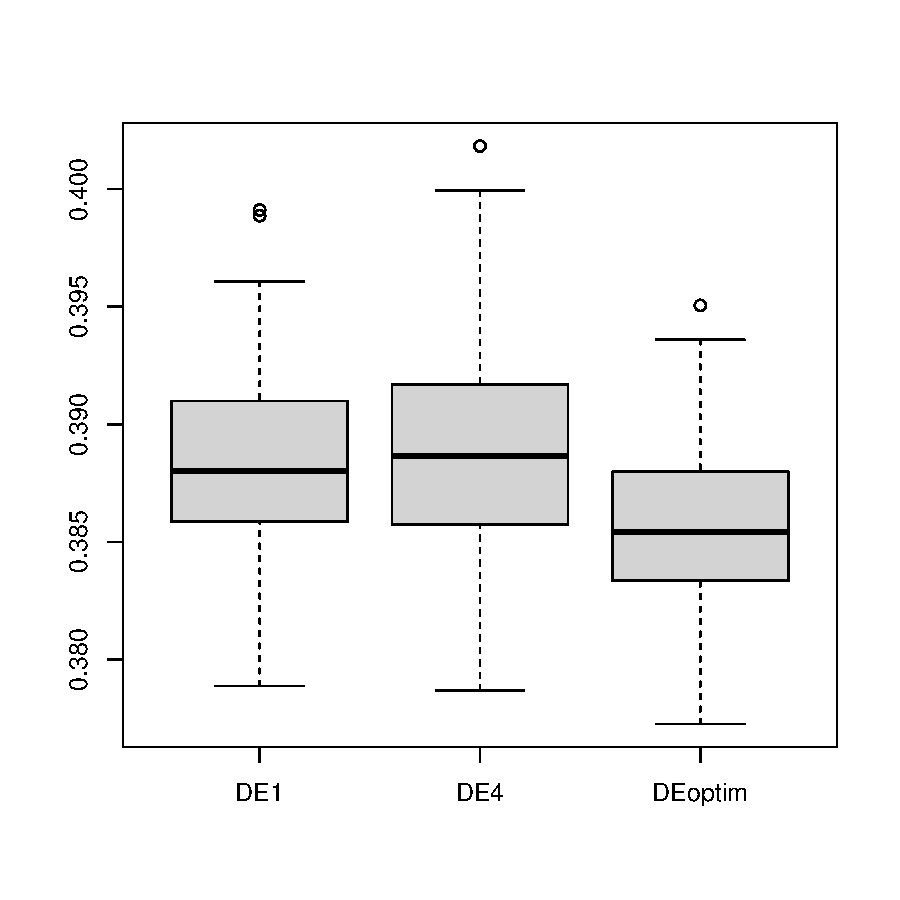
\includegraphics[height=0.5\linewidth]{../chapters/DE/pdfs/boxplots2}
%       \caption{$30\times 3$ as target}
%          %\label{fig:y equals x}
%     \end{figure}
% \end{frame}
% \begin{frame}{Performance of the DE algorithms under three setttings: DE1, DE4 and DEoptim (optimal settings)}
%      \begin{figure}
%          \centering
%          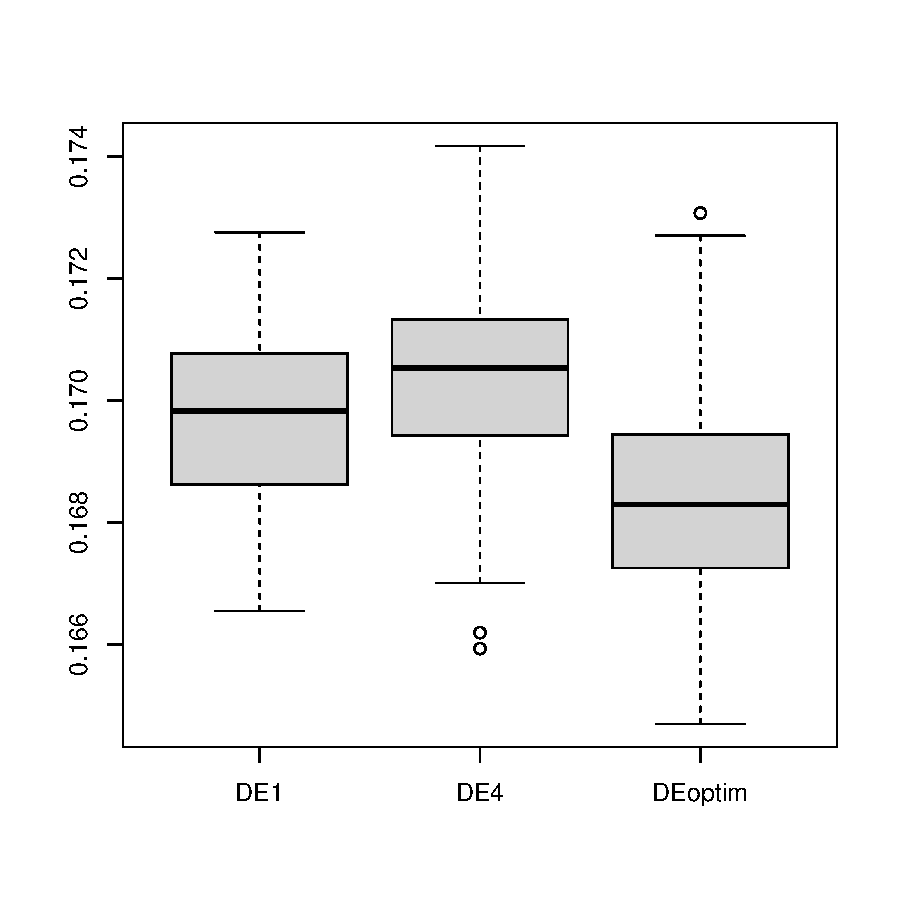
\includegraphics[height=0.5\linewidth]{../chapters/DE/pdfs/boxplots3}
%          \caption{$50\times 5$ as target}
%          %\label{fig:three sin x}
%      \end{figure}
% \end{frame}
% \begin{frame}{Performance of the DE algorithms under three setttings: DE1, DE4 and DEoptim (optimal settings)}
%      \begin{figure}[!h]
%          \centering
%          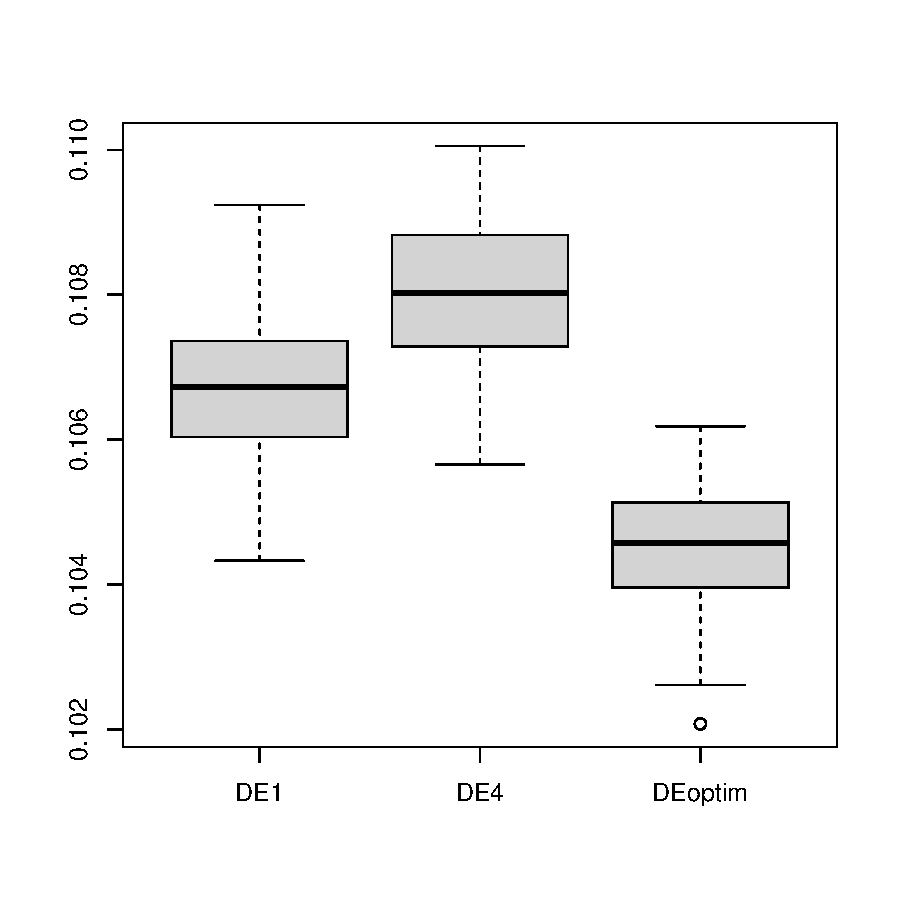
\includegraphics[height=0.5\linewidth]{../chapters/DE/pdfs/boxplots4.pdf}
%          \caption{$70\times 7$ as target}
%          %\label{fig:five over x}
%      \end{figure}
% \end{frame}

\section{Evaluating Space-Filling Designs for Prediction and Sequential Optimization}
\begin{frame}
\begin{itemize}
  \item Objective:  Which space-filling designs offer greater efficiency and robustness for prediction and Optimization
  \item Designs Considered?
  \begin{itemize}
    \item Maximin Design
    \item MaxPro Design
    \item Latin Hypercube Design
    \item Uniform Projection Design
    \item Uniform Design (Only for Prediction)
  \end{itemize}
\end{itemize}
\end{frame}

\subsection{Prediction}
\begin{frame}{Data Generation, Modeling and Evaluation}
\begin{itemize}
  \item Train Data: $64\times 15$, $128\times31$ designs scaled to $[0-1]$
  \item  Test Data: 10,000-run LHD.
  \item Modeling: Kriging Model using Mat\'ern kernel function.
  \item Evaluation: Using Normalized RMSE:
  $$
\text {Normalized RMSE}=\left[\frac{N^{-1} \sum_{i=1}^N\left\{\hat{y}\left(\x_i\right)-y\left(\x_i\right)\right\}^2}{N^{-1} \sum_{i=1}^N\left\{\bar{y}_{train}-y\left(\x_i\right)\right\}^2}\right]^{1 / 2},
$$
\item N = 10000
\item 200 Replications
\end{itemize}
\end{frame}


\begin{frame}
 \begin{figure}
 \centering
 \caption{Borehole - 8D}
 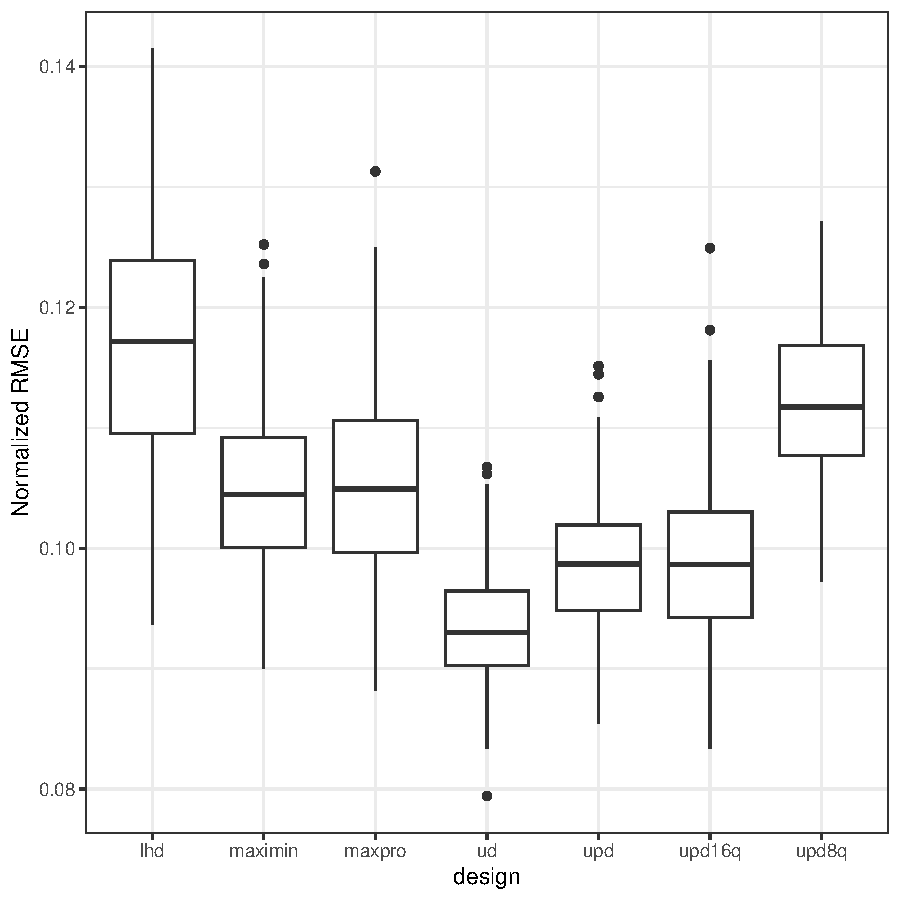
\includegraphics[height=7cm]{../chapters/EGO/pdfs/Borehole_64x15}
 \end{figure}
\end{frame}

% \begin{frame}
% \begin{figure}
% \centering
% \caption{Circuit}
% 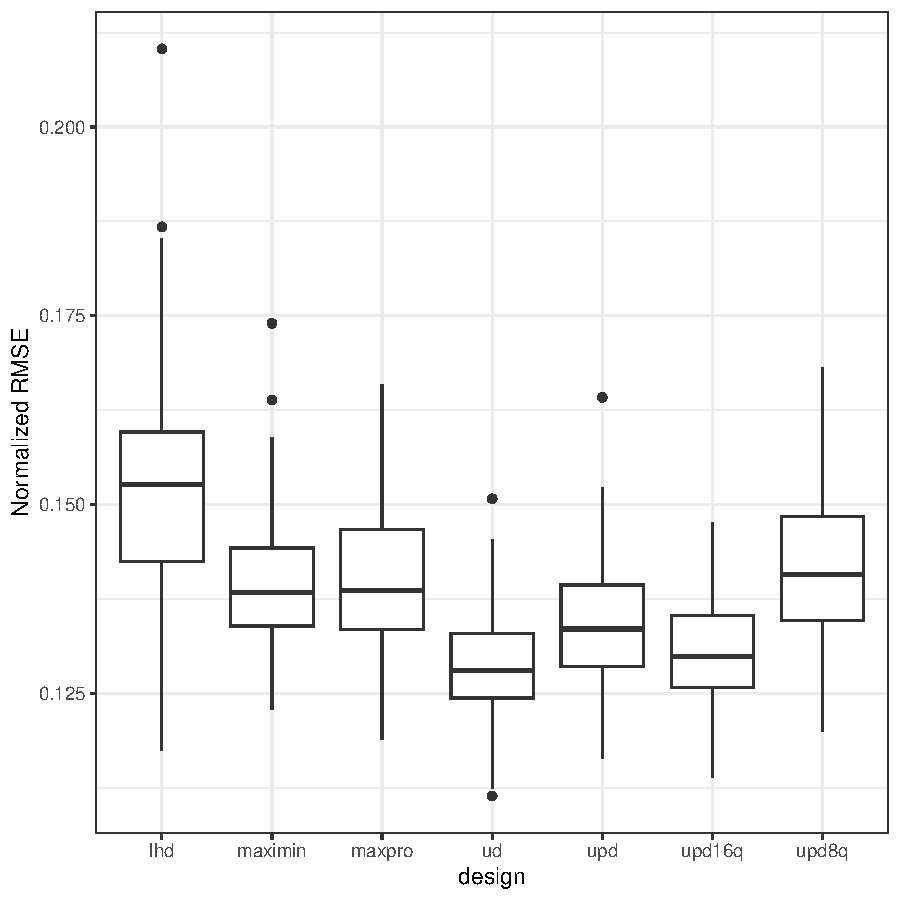
\includegraphics[height=7cm]{../chapters/EGO/pdfs/Circuit_64x15}
% \end{figure}
% \end{frame}

% \begin{frame}
% \begin{figure}
% \centering
% \caption{Currin}
% 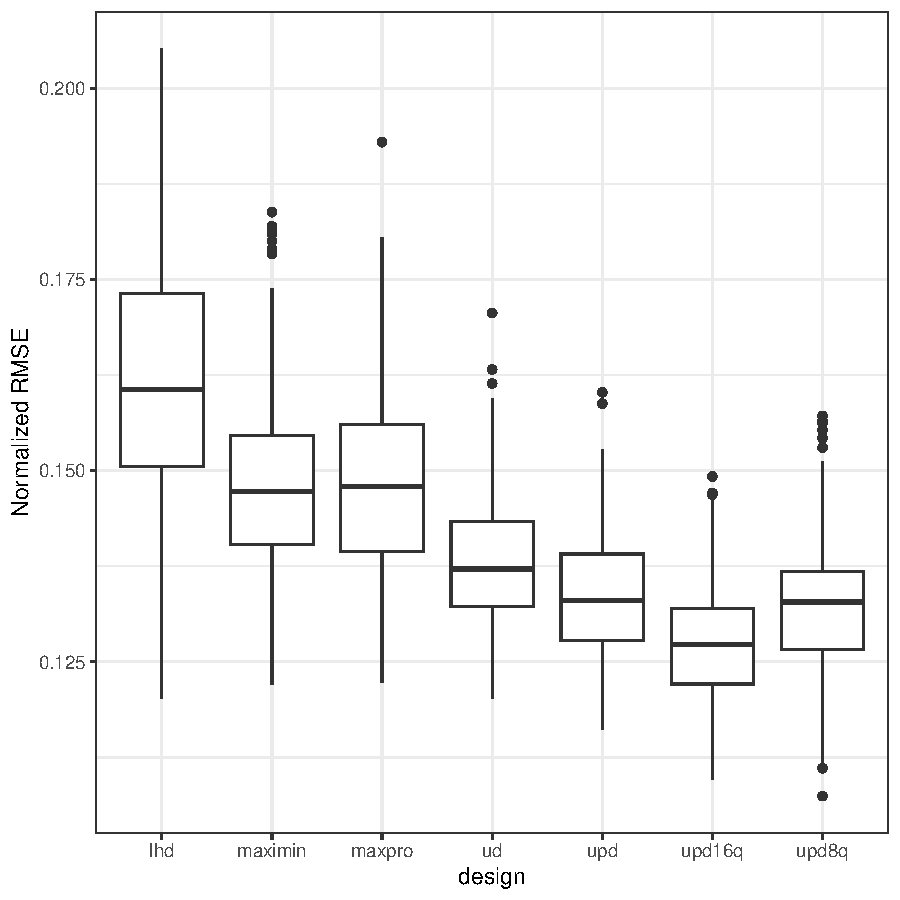
\includegraphics[height=7cm]{../chapters/EGO/pdfs/Currin_64x15}
% \end{figure}
% \end{frame}

\begin{frame}
\begin{figure}
\centering
\caption{Gfunction - 9D}
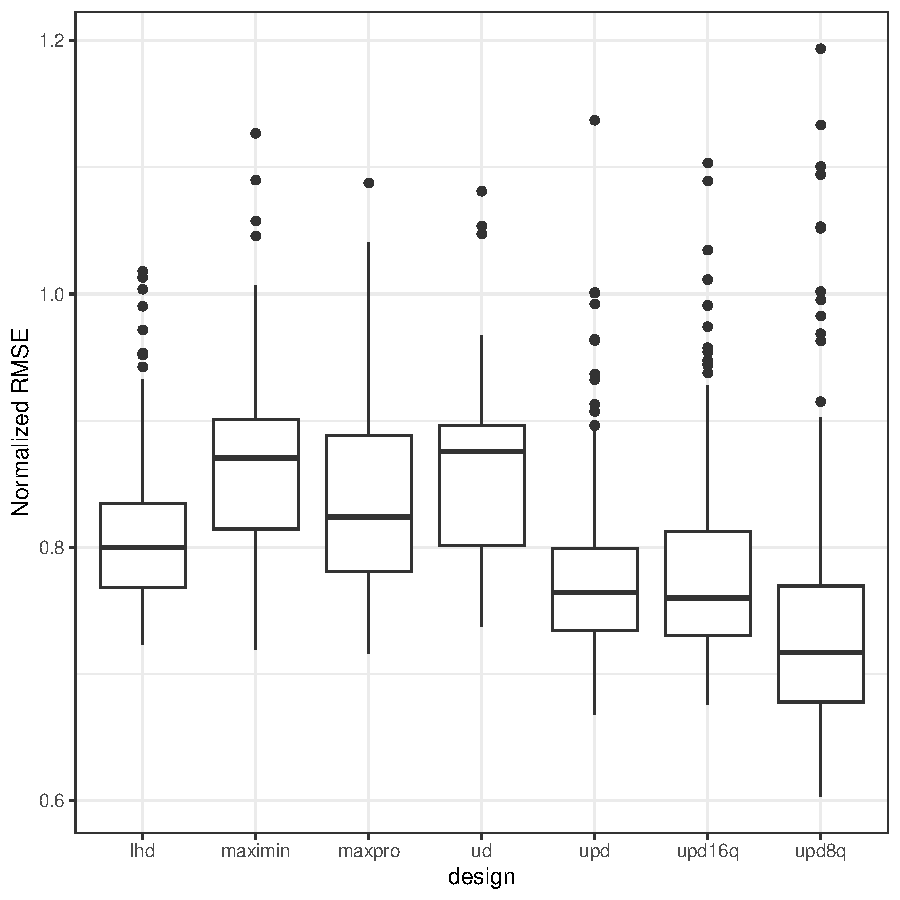
\includegraphics[height=7cm]{../chapters/EGO/pdfs/Gfunction_64x15}
\end{figure}
\end{frame}

% \begin{frame}
% \begin{figure}
% \centering
% \caption{OakleyOhagan}
% 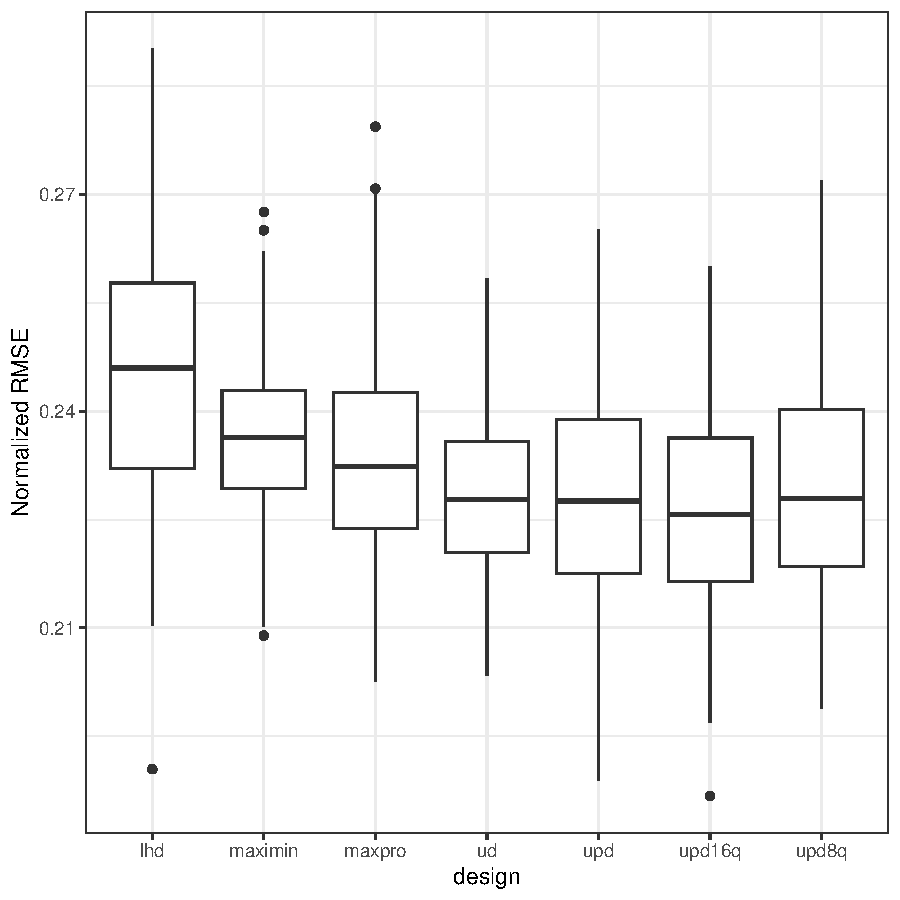
\includegraphics[height=7cm]{../chapters/EGO/pdfs/OakleyOhagan_64x15}
% \end{figure}
% \end{frame}

% \begin{frame}
% \begin{figure}
% \centering
% \caption{Piston}
% 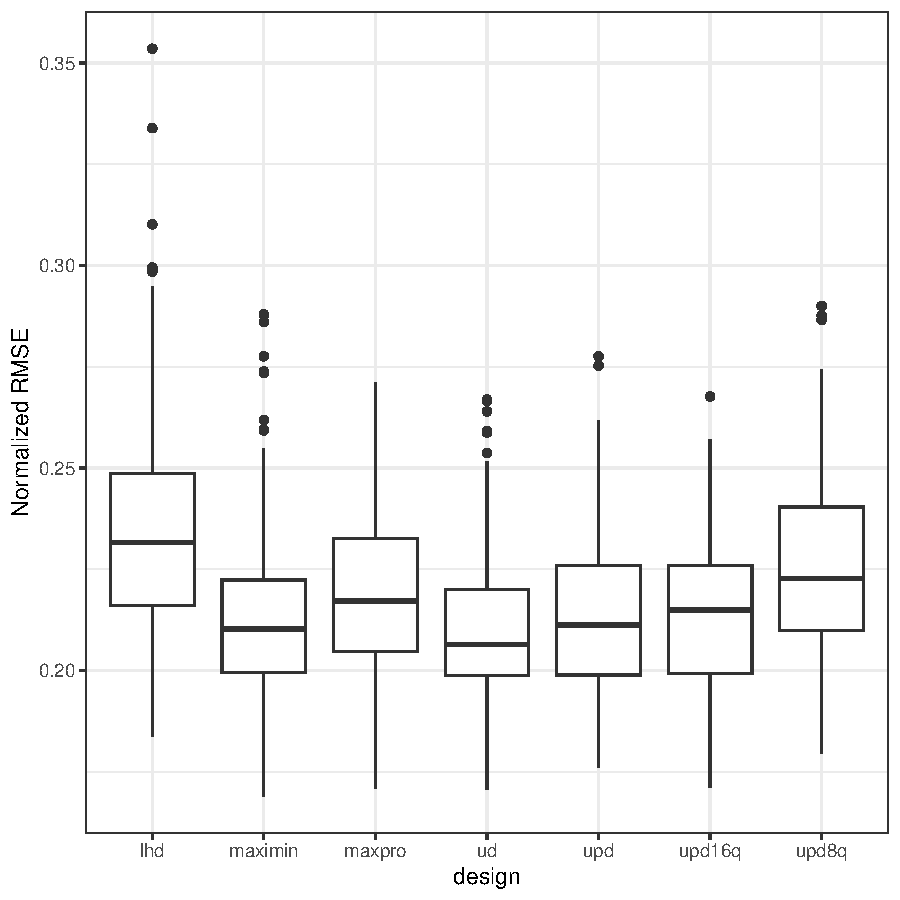
\includegraphics[height=7cm]{../chapters/EGO/pdfs/Piston_64x15}
% \end{figure}
% \end{frame}

\begin{frame}
\begin{figure}
\centering
\caption{4D Rosenbrock}
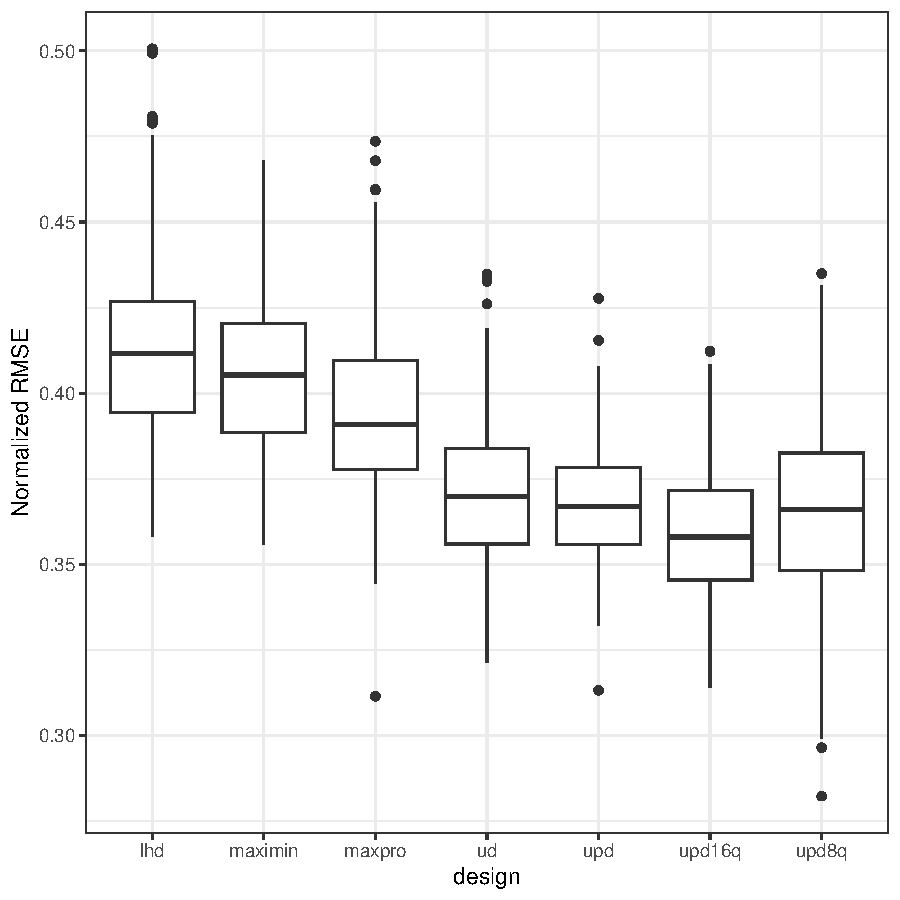
\includegraphics[height=7cm]{../chapters/EGO/pdfs/Rosenbrock4d_64x15}
\end{figure}
\end{frame}

% \begin{frame}
% \begin{figure}
% \centering
% \caption{Wingweight}
% 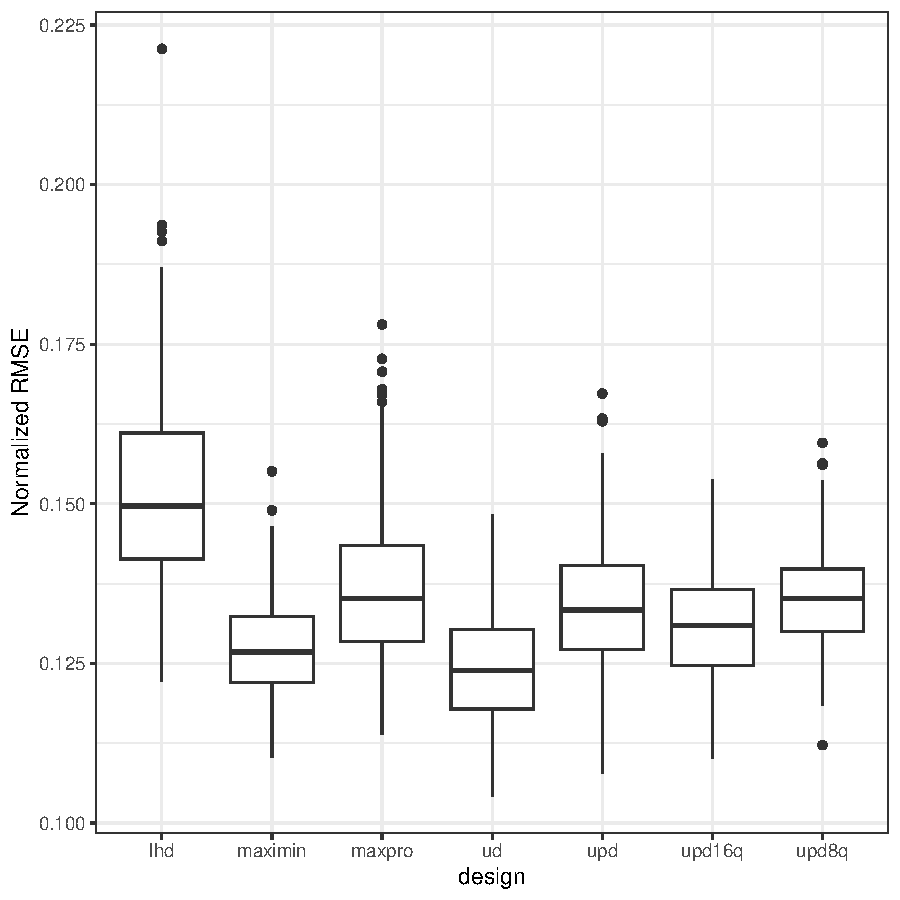
\includegraphics[height=7cm]{../chapters/EGO/pdfs/Wingweight_64x15}
% \end{figure}
% \end{frame}





\subsection{Optimization}
\begin{frame}{Expected Improvement}
\begin{itemize}%[<+->]
    \item Use the Expected Improvement (EI) acquisition function formally given as
    $$
    \mathrm{E}[I(\mathbf{x})] \equiv \mathrm{E}\left[\max \left(f_{\min }-Y, 0\right)\right]
    $$
    \item When $Y\sim N(\hat y, s^2)$ then closed formed is given as

    $$
    \mathrm{E}[I(\mathbf{x})]=\underbrace{\left(f_{\min }-\hat{y}\right) \Phi\left(\frac{f_{\min }-\hat{y}}{s}\right)}_{exploitation} + \underbrace{s \phi\left(\frac{f_{\min }-\hat{y}}{s}\right)}_{exploration}
    $$
    where $\hat y$ is the predictor and $s$ is the standard error at point $\mathbf{x}$, and $\phi(\cdot)$ and $\Phi(\cdot)$ are normal pdf and cdf respectively.
    \parencite{jones1998efficient}

    \item Gives rise to the efficient global Optimization algorithm (EGO)
\end{itemize}
\end{frame}


 \begin{frame}
   \begin{algorithm}[H]
       \caption{EGO algorithm}
       \label{alg:ego2}
       \begin{algorithmic}[1]
           \Require $\X$, $f$ = function to be minimized, $n_{new}$=number of points to add
           \State Evaluate $f$ at the design points $\X$; $\y=f(\X)$
           \State Build a kriging model based on $\X$ and $\y$
           \For{$i$ in $1$ to $n_{new}$}
            \State Find $\x^* \gets \arg\max_{\x}\mathrm{E}[I(\x)]$
            \State Evaluate $\y^* \gets f(\x^*)$
            \State $\X = \X \cup \x^*$ and $\y = \y \cup \y^*$
            \State Update the Kriging Model
           \EndFor
           \State Return $\X, \y$
       \end{algorithmic}
   \end{algorithm}
 \end{frame}


\begin{frame}{EGO 1d Elaboration}
\begin{figure}
    \centering
    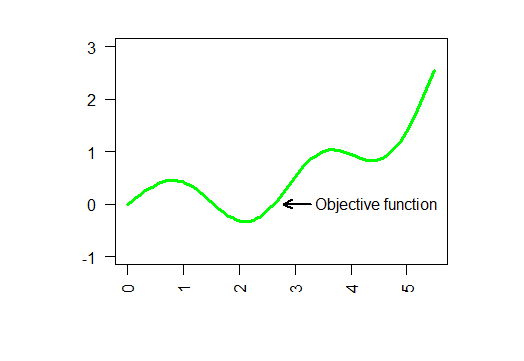
\includegraphics[scale=.7]{images/ego1d/fn1.png}
    \caption{$0.01 x^{3.2} + 0.9  cos(x^{1.1}) sin(x^{1.1})$}
    \label{fig:f1}
\end{figure}
\end{frame}

\begin{frame}{EGO 1d Elaboration}
\begin{figure}
    \centering
    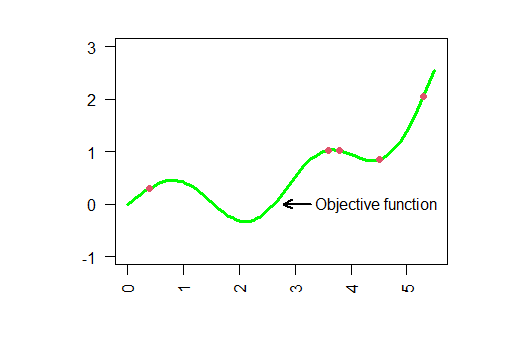
\includegraphics[scale=.7]{images/ego1d/fn2.png}
    %\caption{Caption}
    \label{fig:f2}
\end{figure}
\end{frame}

\begin{frame}{EGO 1d Elaboration}
\begin{figure}
    \centering
    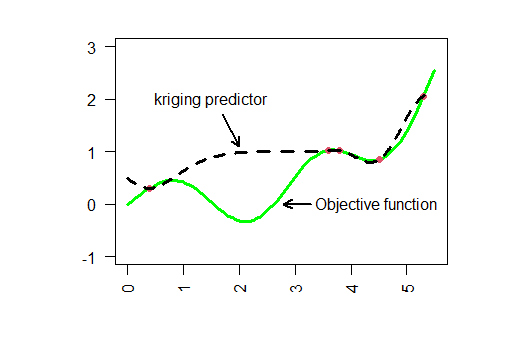
\includegraphics[scale=.7]{images/ego1d/fn3.png}
    %\caption{Caption}
    \label{fig:f3}
\end{figure}
\end{frame}

\begin{frame}{EGO 1d Elaboration}
\begin{figure}
    \centering
    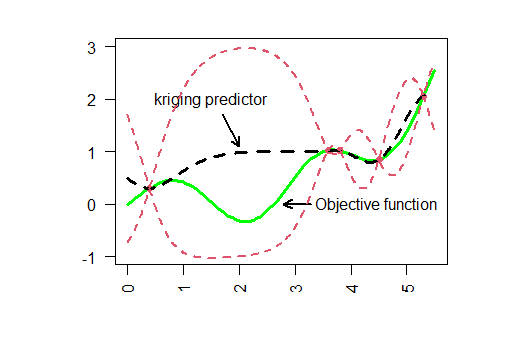
\includegraphics[scale=.7]{images/ego1d/fn4.png}
    %\caption{Caption}
    \label{fig:f4}
\end{figure}
\end{frame}

\begin{frame}{EGO 1d Elaboration}
\begin{figure}
    \centering
    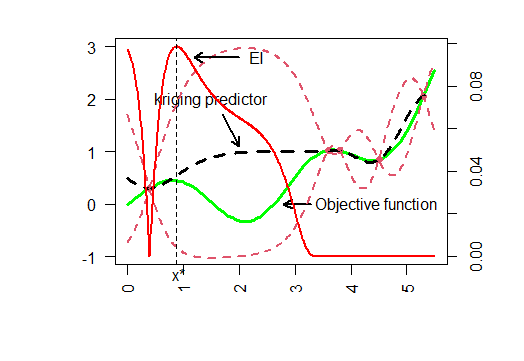
\includegraphics[scale=.7]{images/ego1d/fn5.png}
    %\caption{Caption}
    \label{fig:f5}
\end{figure}
\end{frame}


\begin{frame}{EGO 1d Elaboration}
\begin{figure}
    \centering
    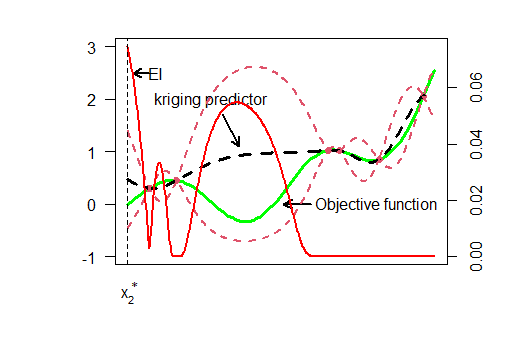
\includegraphics[scale=.7]{images/ego1d/fn6.png}
    %\caption{Caption}
    \label{fig:f6}
\end{figure}
\end{frame}

\begin{frame}{EGO 1d Elaboration}
\begin{figure}
    \centering
    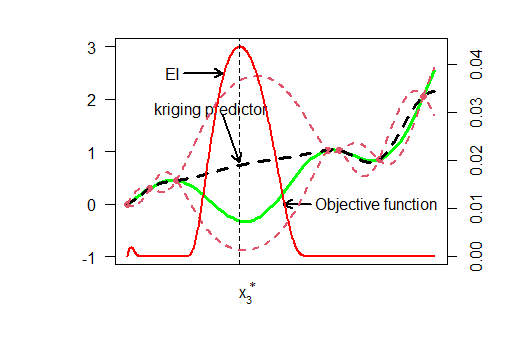
\includegraphics[scale=.7]{images/ego1d/fn7.png}
    %\caption{Caption}
    \label{fig:f7}
\end{figure}
\end{frame}

\begin{frame}{EGO 1d Elaboration}
\begin{figure}
    \centering
    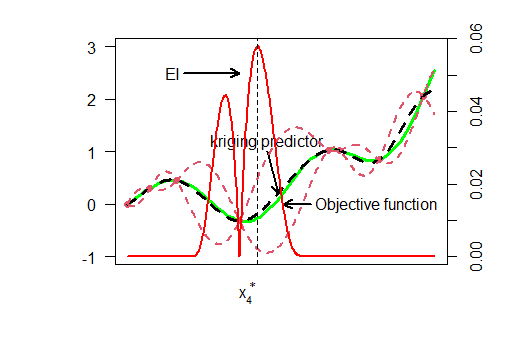
\includegraphics[scale=.7]{images/ego1d/fn8.png}
    %\caption{Caption}
    \label{fig:f8}
\end{figure}
\end{frame}

\begin{frame}{EGO 1d Elaboration}
\begin{figure}
    \centering
    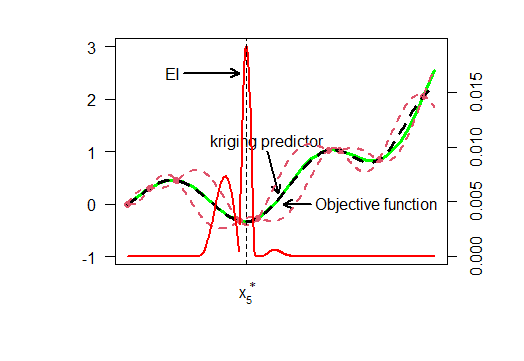
\includegraphics[scale=.7]{images/ego1d/fn9.png}
    %\caption{Caption}
    \label{fig:f9}
\end{figure}
\end{frame}

\begin{frame}{EGO 1d Elaboration}
\begin{figure}
    \centering
    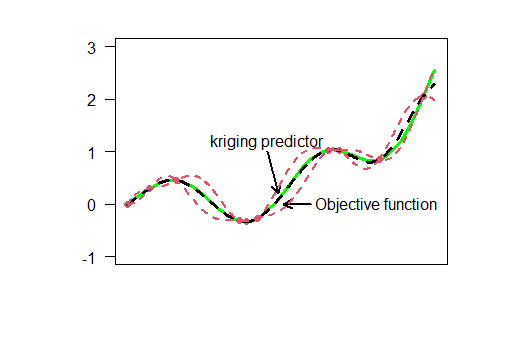
\includegraphics[scale=.7]{images/ego1d/fn10.png}
    %\caption{Caption}
    \label{fig:f10}
\end{figure}
\end{frame}

\subsection{Results}
\begin{frame}{Initial Design Minimization Path}
\begin{figure}
\centering
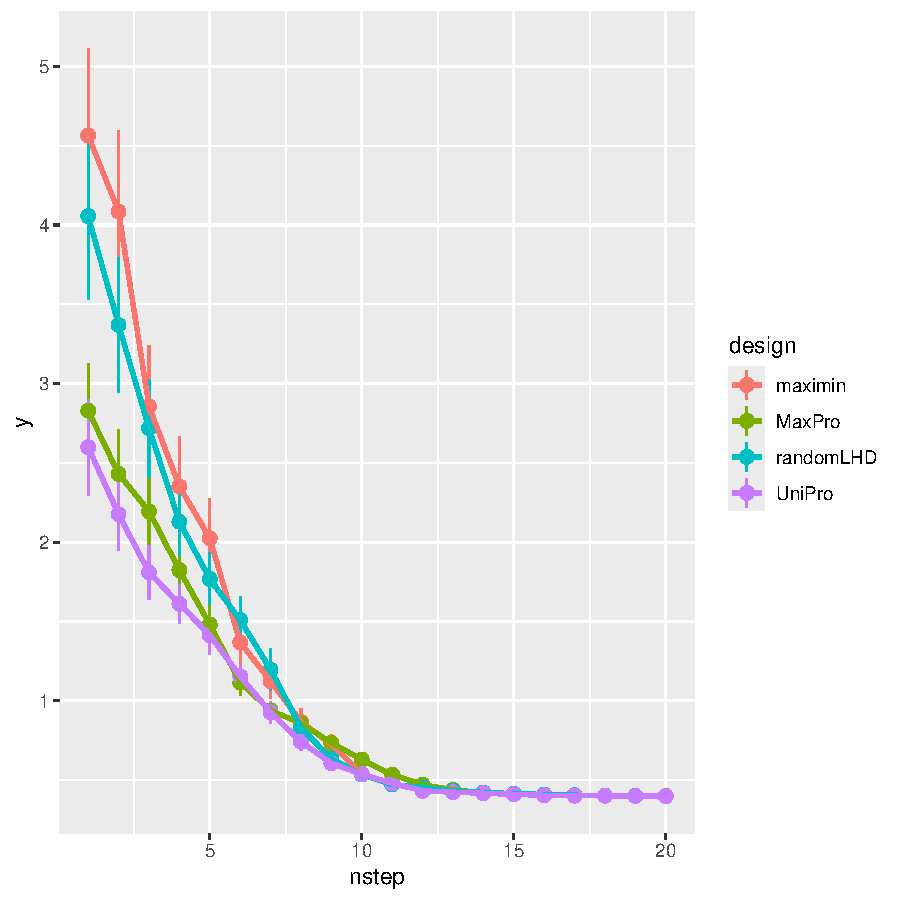
\includegraphics[height=7cm]{../chapters/EGO/pdfs/branin_lineplot1}
\caption{Branin (2D)}
\end{figure}
\end{frame}

\begin{frame}{Initial Design Minimization Path}
\begin{figure}
\centering
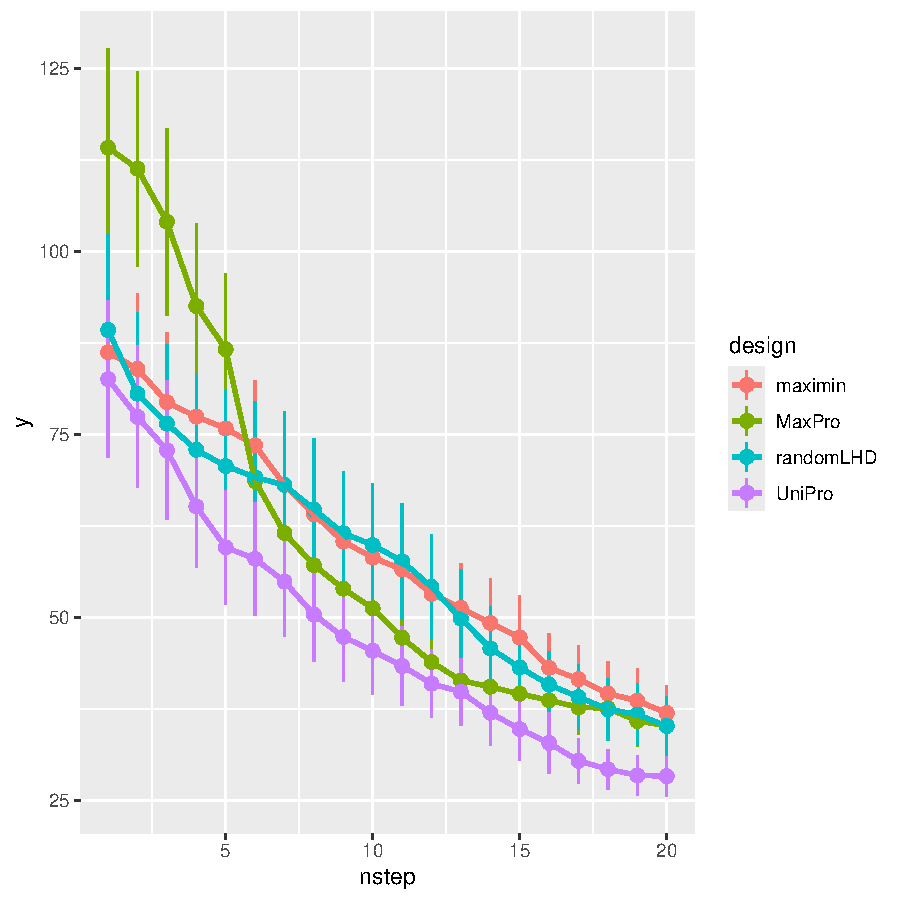
\includegraphics[height=7cm]{../chapters/EGO/pdfs/goldpr_lineplot1}
\caption{Goldstein-Price (2D)}
\end{figure}
\end{frame}

% \begin{frame}{Initial Design Minimization Path}
% \begin{figure}
% \centering
% 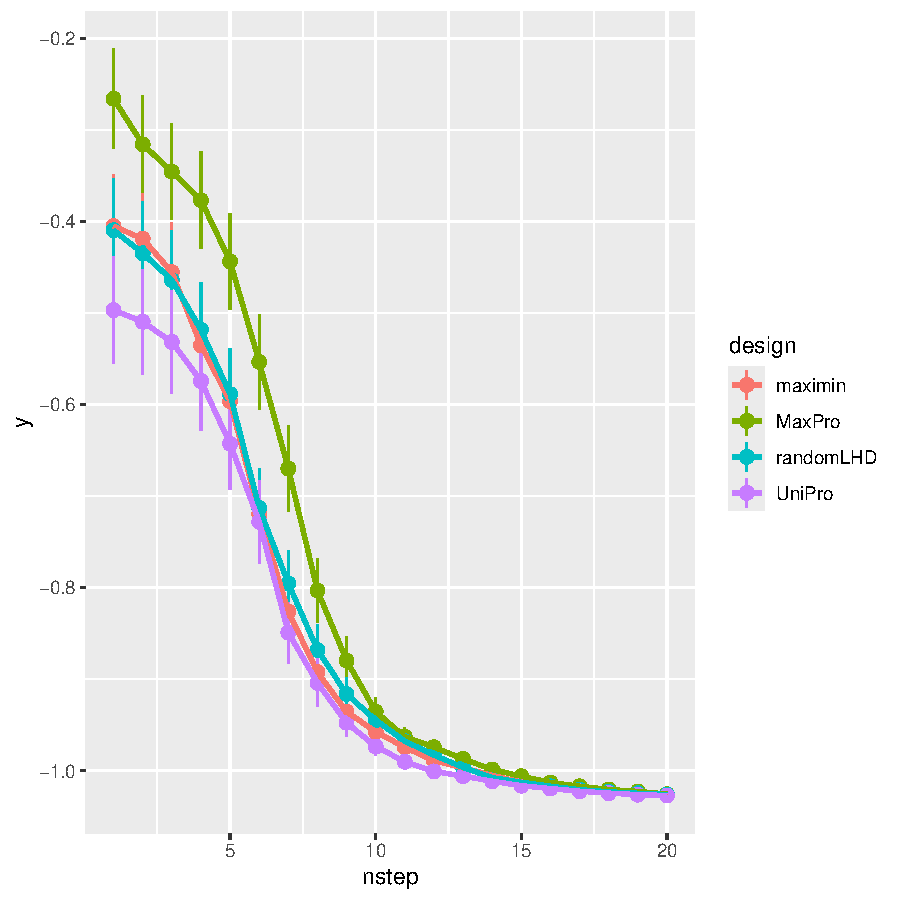
\includegraphics[height=7]{../chapters/EGO/pdfs/camel6_lineplot1}
% \caption {Camel Six (2D)}
% \end{minipage}
% \end{frame}

\begin{frame}{Initial Design Minimization Path}
\begin{minipage}{0.32\textwidth}
\centering
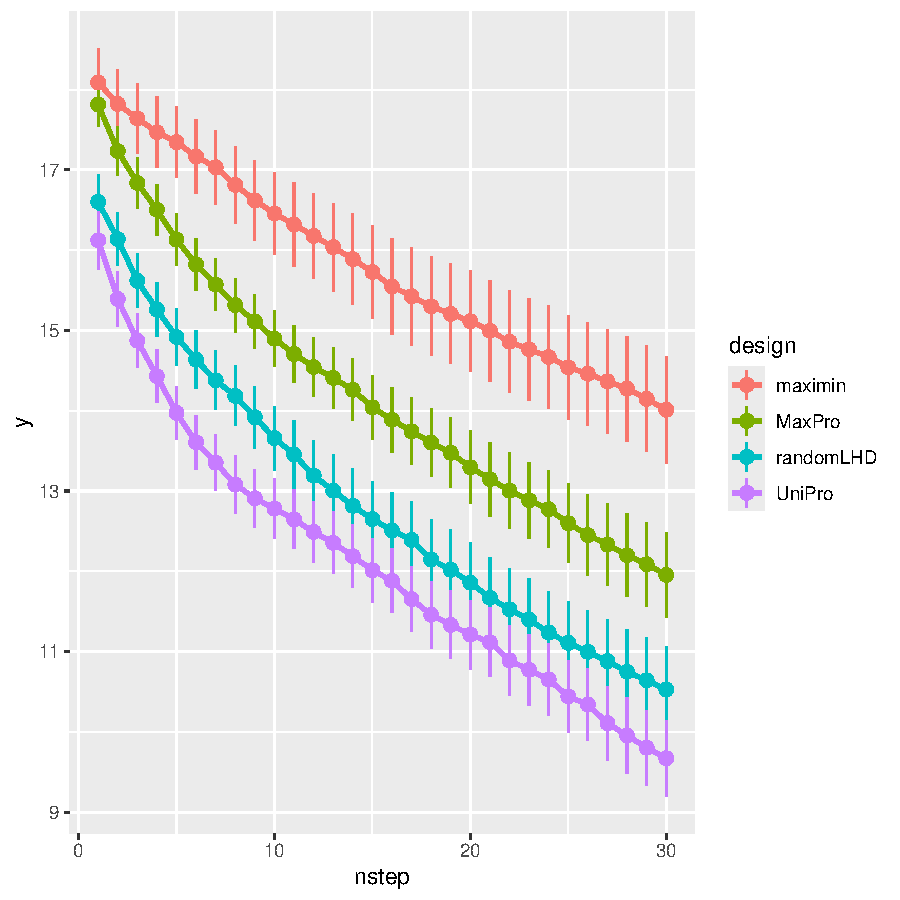
\includegraphics[width=\textwidth]{../chapters/EGO/pdfs/ackley6_lineplot1}
\small{6D Ackley}
\end{minipage}
\hfill
\begin{minipage}{0.32\textwidth}
\centering
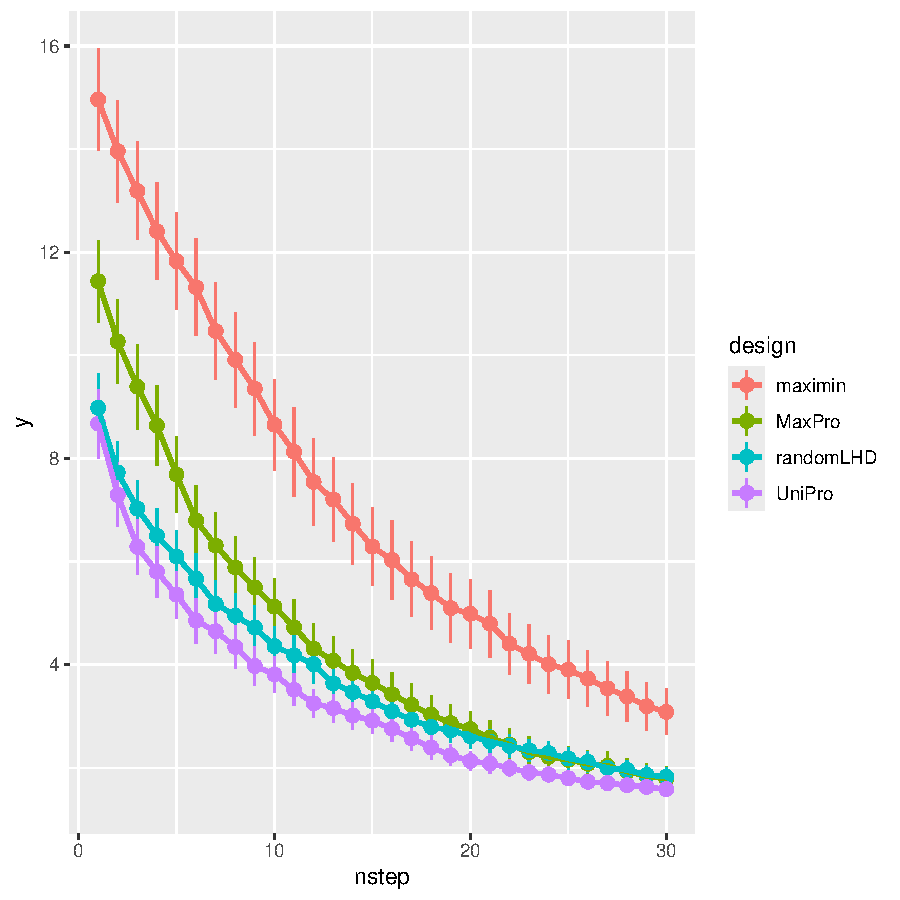
\includegraphics[width=\textwidth]{../chapters/EGO/pdfs/levy6_lineplot1}
\small {6D Levy}
\end{minipage}
\hfill
\begin{minipage}{0.32\textwidth}
\centering
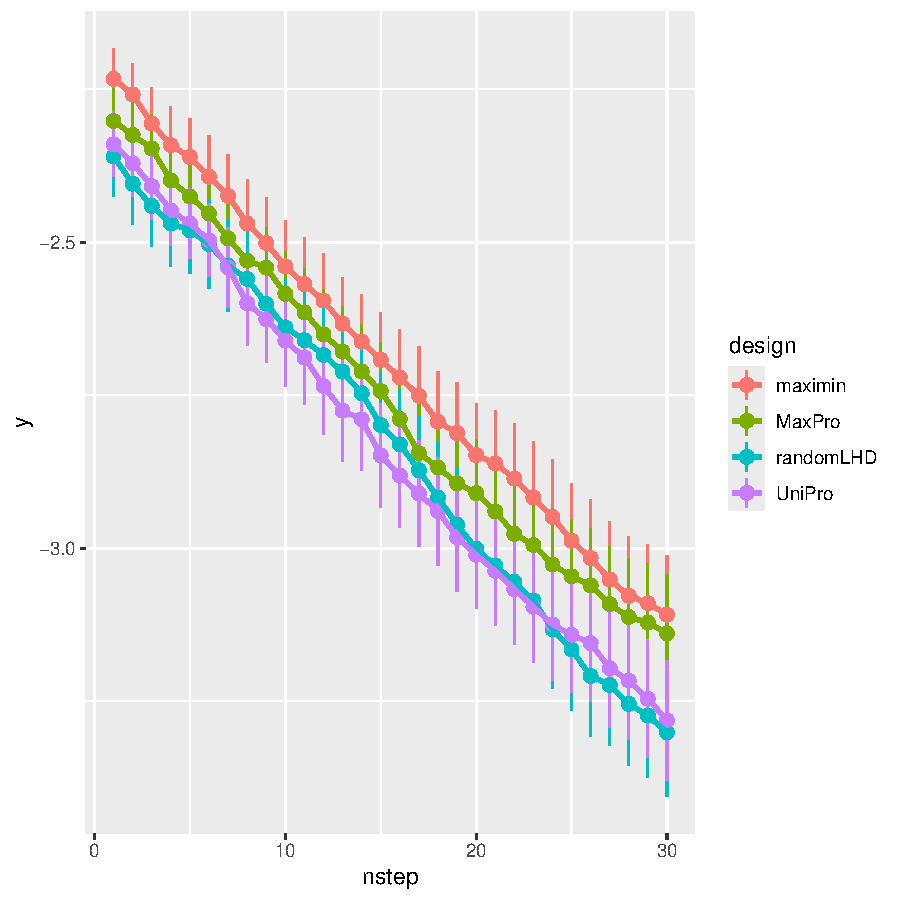
\includegraphics[width=\textwidth]{../chapters/EGO/pdfs/michal6_lineplot1}
\small{6D Michalewicz}
\end{minipage}
\end{frame}

\begin{frame}{Initial Design Minimization Path}
\begin{minipage}{0.32\textwidth}
\centering
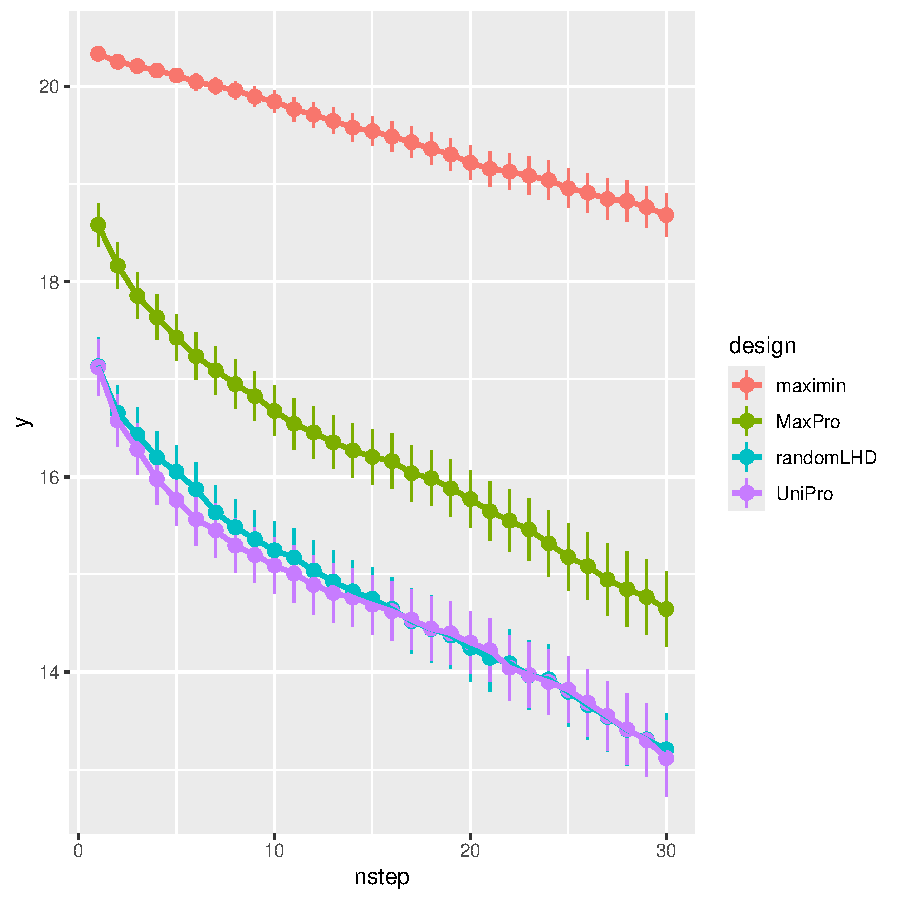
\includegraphics[width=\textwidth]{../chapters/EGO/pdfs/ackley8_lineplot1}
\small {8D Ackley}
\end{minipage}
\hfill
\begin{minipage}{0.32\textwidth}
\centering
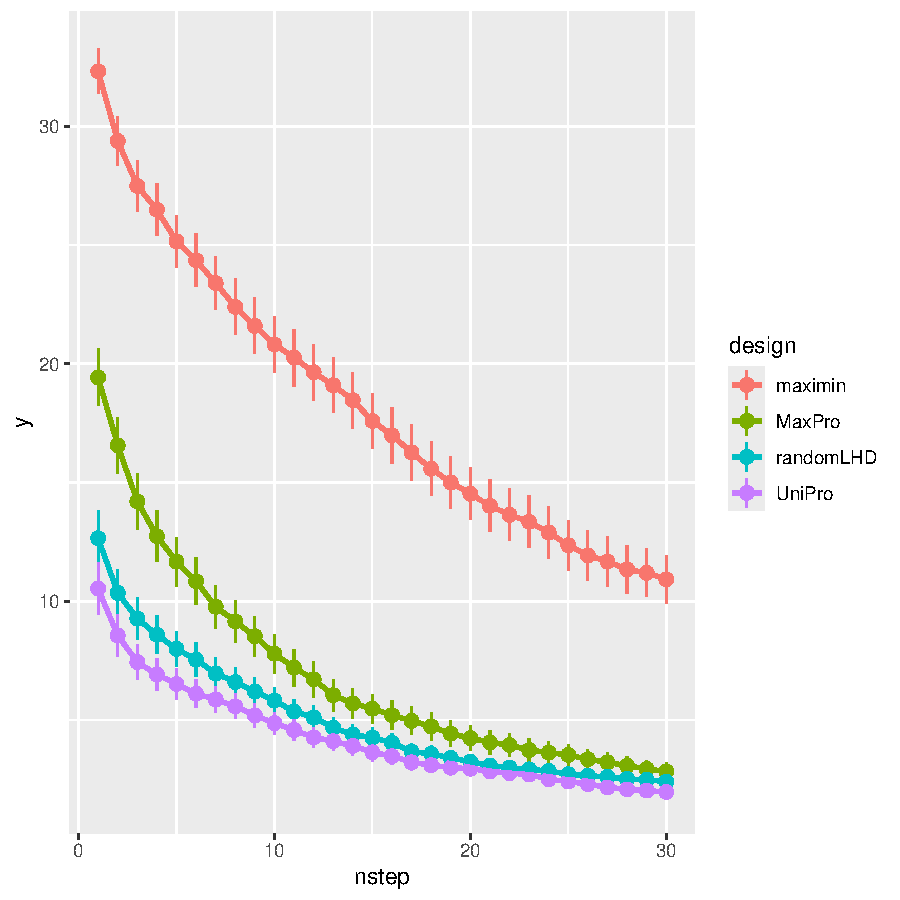
\includegraphics[width=\textwidth]{../chapters/EGO/pdfs/levy8_lineplot1}
\small {8D Levy}
\end{minipage}
\hfill
\begin{minipage}{0.32\textwidth}
\centering
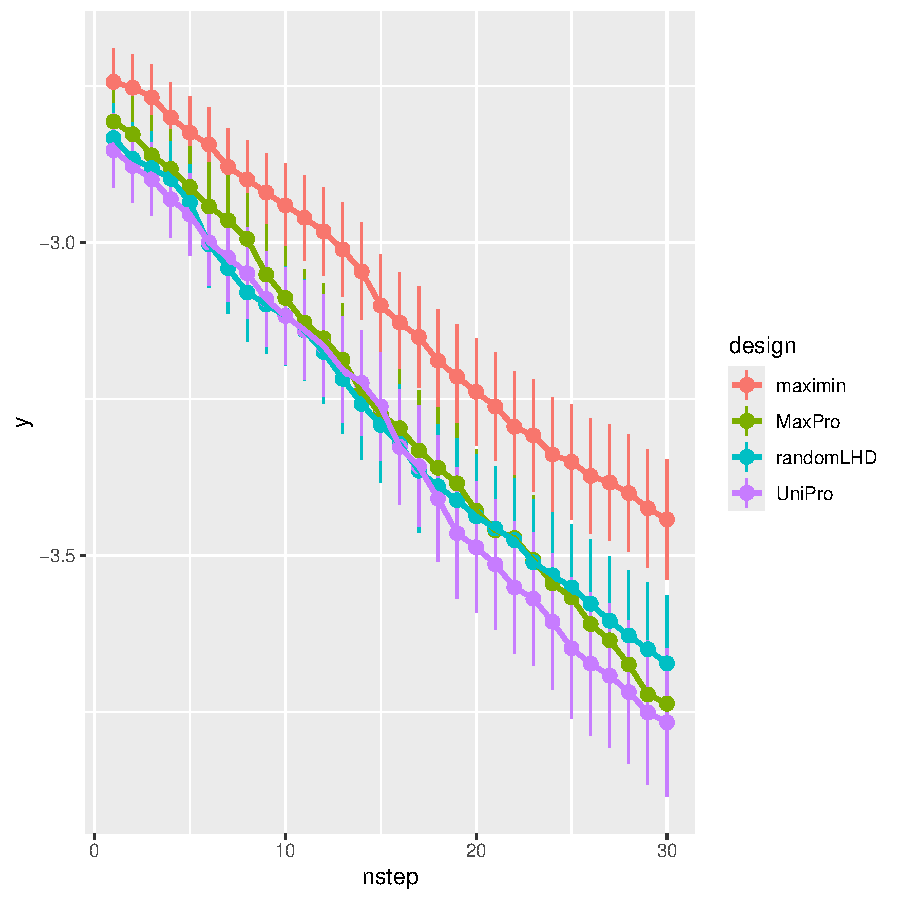
\includegraphics[width=\textwidth]{../chapters/EGO/pdfs/michal8_lineplot1}
\small {8D Michalewicz}
\end{minipage}
\end{frame}




\section{Kriging Based Sequential Region Shrinkage with EGO for  Hyperparameter Optimization}

% \begin{frame}{Background}
% \begin{itemize}
%     \item Problem of choosing a set of optimal hyperparameters for a learning algorithm
%     \item Performance of these algorithms highly depends on their hyperparameter configurations \parencite{feurer2019hyperparameter} and may flactuate drastically under different architectures\parencite{liu2018darts}.
%     \item Two lines of work \begin{enumerate}
%         \item Model free methods - Grid Search, Random Search
%         \item Model Based methods - fitting a surrogate model eg Kriging and optimize -- Bayesian Optimization (BO)
%     \end{enumerate}
%     \item Preference to Model based method as one can achieve  a global or near global optimum using fewer model evaluations  \parencite{yaohui2017kriging}.
% \end{itemize}
% \end{frame}

% \subsection{Problem Formulation}
% \begin{frame}{Problem Formulation}
%     \begin{itemize}[<+->]
%         \item Unknown and computationally expensive  objective function ie black-box function.
%         \item Cannot be optimized using gradient based methods -- Score function intractable. The
%          way forward? Use Bayesian Optimization \parencite{pelikan1999boa}\\
%          $$x^* = \underset{x\in A}{\arg\max} f(x)$$
%          where $A$ denotes the search space of $x$.
%          \item The principle of BO is to
% combine the prior distribution of $f(x)$ with the sample information to obtain the posterior of the  function; which is maximized according to a chosen acquisition function.
%     \end{itemize}
% \end{frame}



\begin{frame}{Efficient Global Optimization -- Limitations}
\begin{itemize}
    \item Slow Convergence as each iteration is over the entire search space
    \item Struggles to scale with dimension %\parencite{diouane2022trego}.
\end{itemize}
\end{frame}



\begin{frame}{Objective}
    Propose a method that focuses on a specific region of interest within the entire domain space in each iteration.
    Use the proposed method to optimize the UniPro construction.
\end{frame}
\subsection{Our Method}
% \begin{frame}{Kriging based Region shrinkage for HPO}
%     \begin{itemize}
%         \item Takes into consideration a controlled parameter $\rho\in(0, 1)$
%         \item Uses $\rho$ to determine the number of top $100\rho\%$ points from the data.
%         \item Computes region of interest (ROI) boundary using the top $100\rho \%$ points as the minimum and maximum of each dimension.
%         \item Shift the region to be centered at the current best $x_t^*$
%         \item In case the ROI falls outside the function domain, constrain the ROI boundaries to be within the domain.
%         \item carry out EGO and add $m$ points.
%         \item When converged, set the ROI to the entire domain space and carry out the EGO one more time.
%     \end{itemize}
% \end{frame}

\begin{frame}{Kriging based Region shrinkage for HPO}
  \begin{algorithm}[H]
      \caption{Sequential Region Shrinkage Method}
      \label{alg:srs}
      \begin{algorithmic}[1]
        \Require $\X$, $f$, $\Omega$ = domain, $n_{new}$, $\rho$
       \State Evaluate $f$ at the design points $\X$; $\y \gets f(\X)$
       \State Build a Kriging model based on $\X$ and $\y$
       \State Set the region of interest (ROI) $\Omega' \gets \Omega$ (initial domain)
       \While{stopping criteria not met}
         \State Run EGO within the domain $\Omega'$ to obtain the next $n_{new}$ points
         \State Update $\X$ and $\y$ with the new points
         \State Update the Kriging model
         \State Determine the new ROI $\Omega' \gets \text{ROI}(\X, \y, \rho)$
         \If{small or no improvement (unsuccessful iteration)}
           \State Restore the original domain: $\Omega' \gets \Omega$
         \EndIf
       \EndWhile
       \State Return $\X$, $\y$
     \end{algorithmic}
  \end{algorithm}
 \end{frame}

\begin{frame}
\begin{algorithm}[H]
    \caption{Determine Region of Interest (ROI)}\label{alg:roi}
    \begin{algorithmic}[1]
        \Require $\X$, $\Omega$ = domain, $\y$, $\rho$.
        \State $\tau \gets \text{indices of the top } 100\rho\% \text{ of } \y$.
        \State Select points in $\X$ associated with $\tau$.
        \State Find the best point $\x^*$ that minimizes the objective function  %:= \arg\min{\y}$
        \State {Determine the lower and upper bounds for points associated with $\tau$;  set $L_j :=  \min_{i \in \tau} x_{ij}$ and $ U_j :=  \max_{i \in \tau} x_{ij}$ for each $j=1,\ldots, d$}
        \State Set $\mathbf{D} := (\mathbf{U} - \mathbf{L})/2$, where $\mathbf{U}=(U_1, \ldots, U_d)$ and $\mathbf{L}=(L_1, \ldots, L_d)$.
        \State Set {$\Omega' =  \left\{\x^* - \mathbf{D},  \x^* + \mathbf{D} \right\} \cap \Omega$.}
        \State \Return $\Omega'$.
    \end{algorithmic}
\end{algorithm}

\end{frame}


\begin{frame}{Example of ROI Determination Using Branin}
    \begin{figure}
        \centering
        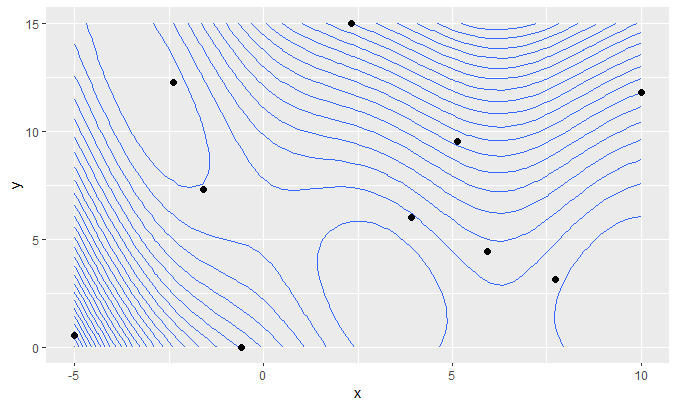
\includegraphics[scale=.5]{images/branin/R0.png}
        \caption{Initial design points}
        \label{fig:branin0}
    \end{figure}
\end{frame}
\begin{frame}{Example of ROI Determination Using Branin}
    \begin{figure}
        \centering
        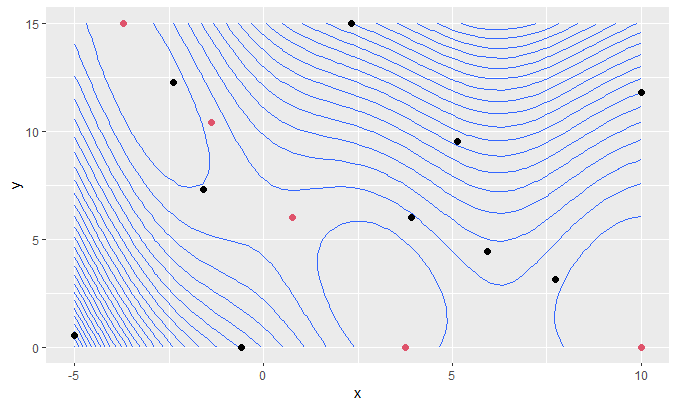
\includegraphics[scale=.5]{images/branin/R1.png}
        \caption{5 points added using EGO}
        \label{fig:branin1}
    \end{figure}
\end{frame}
\begin{frame}{Example of ROI Determination Using Branin}
    \begin{figure}
        \centering
        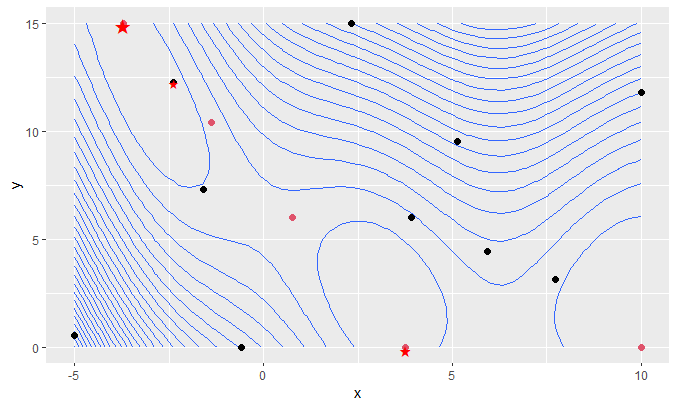
\includegraphics[scale=.5]{images/branin/R2.png}
        \caption{The best 3 points ie $\rho = 20\%$}
        \label{fig:branin2}
    \end{figure}
\end{frame}
\begin{frame}{Example of ROI Determination Using Branin}
    \begin{figure}
        \centering
        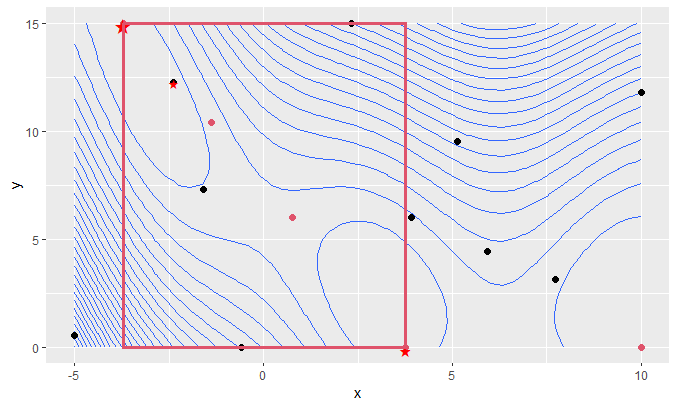
\includegraphics[scale=.5]{images/branin/R3.png}
        \caption{Region containing the best 20\% of the points}
        \label{fig:branin3}
    \end{figure}
\end{frame}
\begin{frame}{Example of ROI Determination Using Branin}
    \begin{figure}
        \centering
        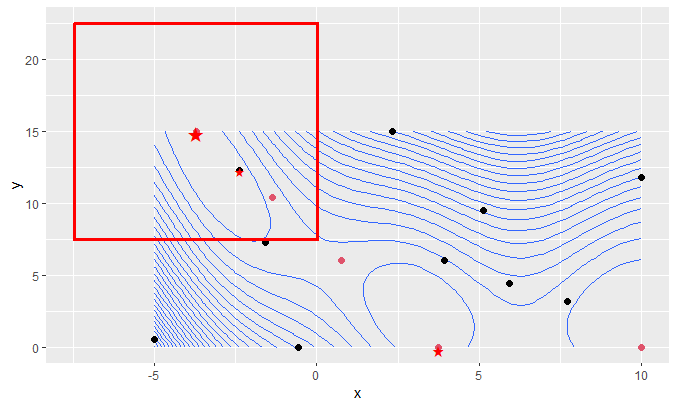
\includegraphics[scale=.5]{images/branin/R4.png}
        \caption{ROI centered at the current best point}
        \label{fig:branin4}
    \end{figure}
\end{frame}
\begin{frame}{Example of ROI Determination Using Branin}
    \begin{figure}
        \centering
        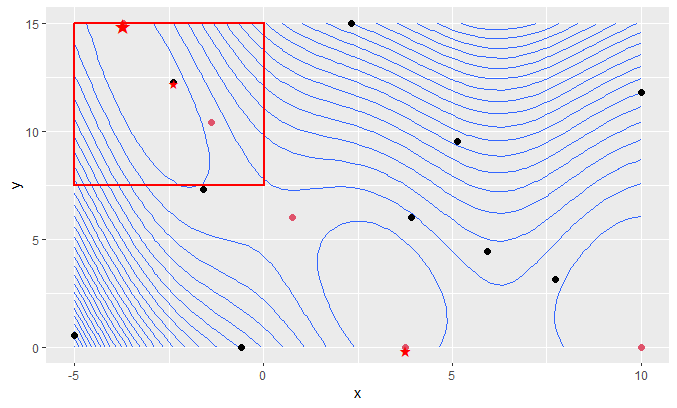
\includegraphics[scale=.5]{images/branin/R5.png}
        \caption{ROI constrained to be within the function domain}
        \label{fig:branin5}
    \end{figure}
\end{frame}
\begin{frame}{Why Restore the Region?}
    \begin{itemize}
        \item Once converged, the current optimum is optimal only for the ROI
        \item We need to check as to whether its optimal for the entire search space
        \item Restore the ROI to the entire function domain and carry out EGO
        \item Check as to whether you converge to the current optimal
        item Continue with the optimization if you obtain a better point than the current point
    \end{itemize}
\end{frame}
\subsection{Results}

% \begin{frame}{Results}
% \begin{minipage}{0.32\textwidth}
% \centering
% 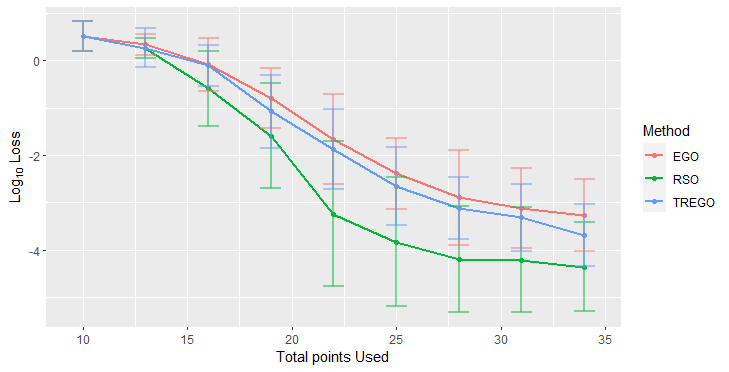
\includegraphics[width=\textwidth]{../chapters/RSO/pdfs/branin_error.png}
% \small {Branin}
% \end{minipage}
% \begin{minipage}{0.32\textwidth}
% \centering
% 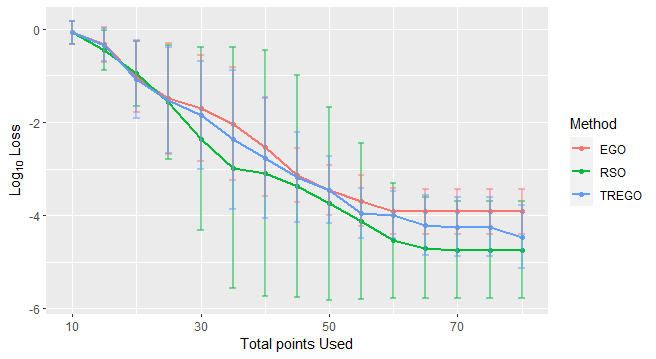
\includegraphics[width=\textwidth]{../chapters/RSO/pdfs/hart4.png}
% \small {Hartmann4}
% \end{minipage}
% \begin{minipage}{0.32\textwidth}
% \centering
% 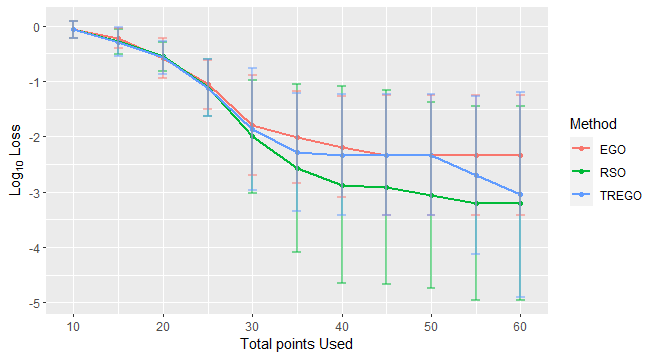
\includegraphics[width=\textwidth]{../chapters/RSO/pdfs/hart6.png}
% \small {Hartmann6}
% \end{minipage}
% \end{frame}

\begin{frame}{Results -- Branin (2D)}
\begin{figure}
\centering
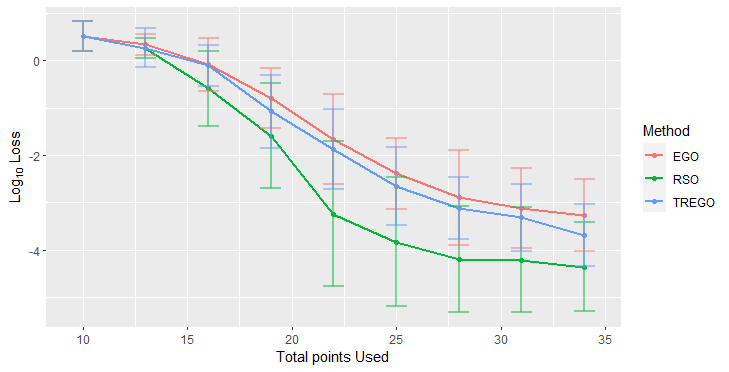
\includegraphics[height=7cm]{../chapters/RSO/pdfs/branin_error.png}
\small {Branin}
\end{figure}
\end{frame}

\begin{frame}{Results -- Hartmann4 (4D)}
\begin{figure}
\centering
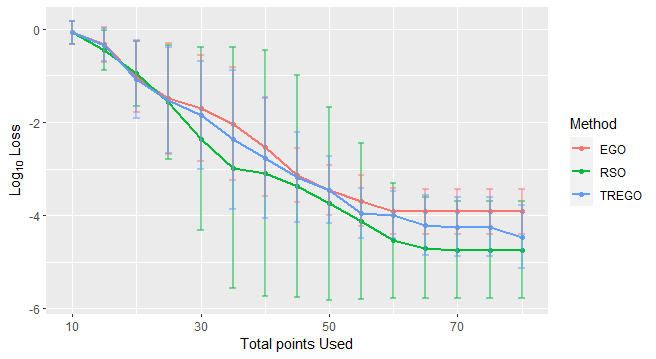
\includegraphics[height=7cm]{../chapters/RSO/pdfs/hart4.png}
\small {Hartmann4}
\end{figure}
\end{frame}
\begin{frame}{Results -- Hartmann6 (6D)}
\begin{figure}
\centering
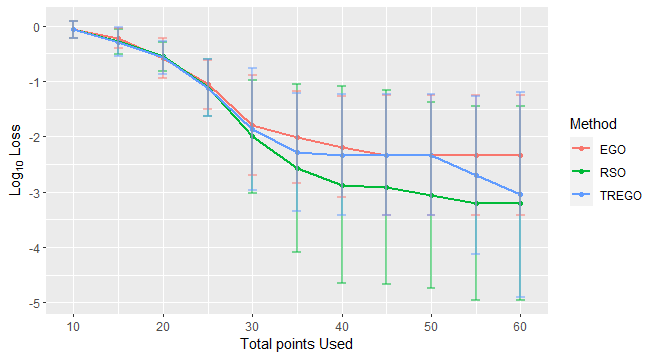
\includegraphics[height=7cm]{../chapters/RSO/pdfs/hart6.png}
\small {Hartmann6}
\end{figure}
\end{frame}


\begin{frame}{Methods Minimization Path}
\begin{minipage}{0.32\textwidth}
\centering
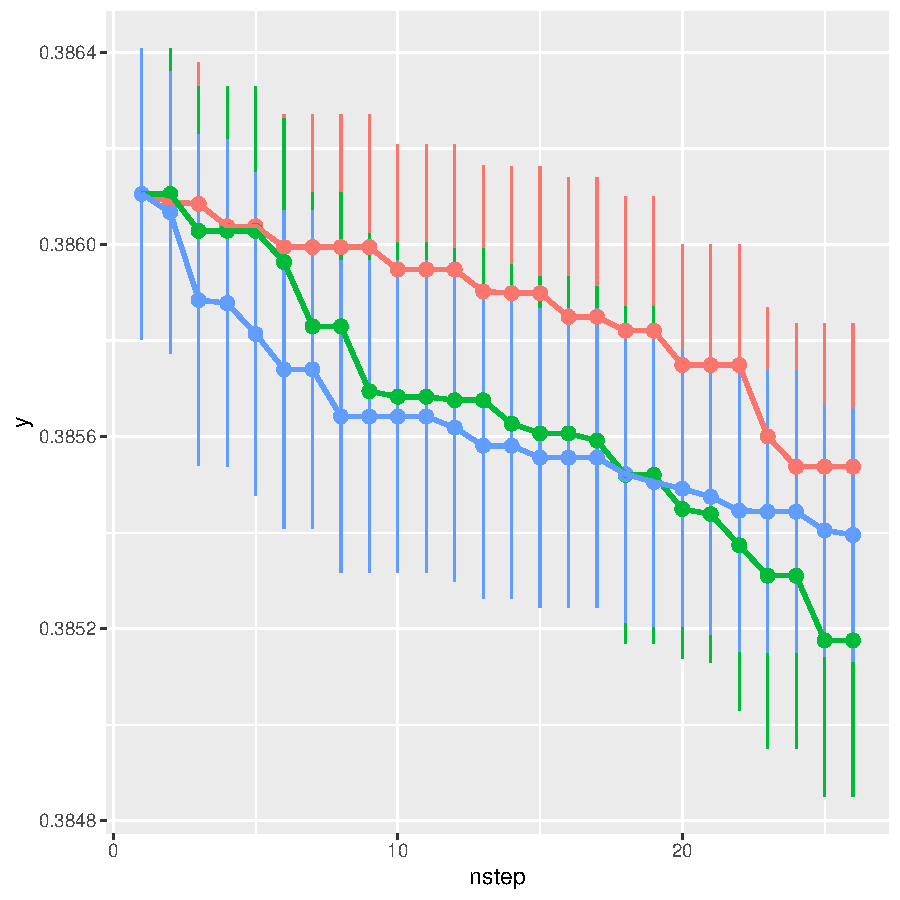
\includegraphics[]{../chapters/RSO/pdfs/results30x3}
\small {$30\times 3$}
\end{minipage}
\begin{minipage}{0.32\textwidth}
\centering
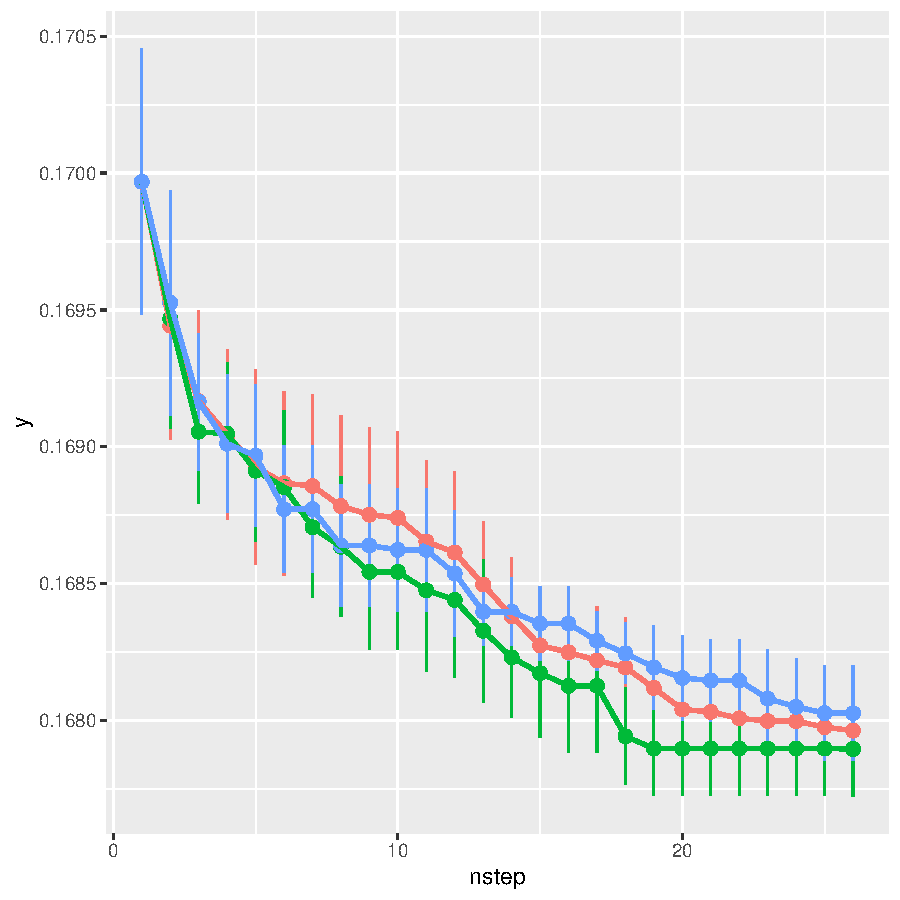
\includegraphics[]{../chapters/RSO/pdfs/results50x5}
\small {$50\times 5$}
\end{minipage}
\begin{minipage}{0.32\textwidth}
\centering
\includegraphics[]{../chapters/RSO/pdfs/results70x7}
\small {$70\times 7$}
\end{minipage}
\end{frame}


\begin{frame}{Methods Comparison Boxplots}
\begin{minipage}{0.32\textwidth}
   \centering
   \includegraphics[]{../chapters/RSO/pdfs/boxplots2}
   \small {$30\times 3$ as target}
\end{minipage}
\begin{minipage}{0.32\textwidth}
   \centering
   \includegraphics[]{../chapters/RSO/pdfs/boxplots3}
   \small{$50\times 5$ as target}
\end{minipage}
\begin{minipage}{0.32\textwidth}
   \centering
   \includegraphics[]{../chapters/RSO/pdfs/boxplots4}
   \small{$70\times 7$ as target}
\end{minipage}
\end{frame}


\begin{frame}{Contributions}
\begin{itemize}
  \item Study showing efficiency of UniPro
  \item Novel algorithm for generalized optimization
  \item Package to generate efficient UniPro designs
\end{itemize}
\end{frame}

% \begin{frame}{Pros and Cons}
% \begin{itemize}
%     \item Needs fewer number of runs than grid search.
%     %\item Depends on the initial design (not shown)
%     \item  only converge to one optimum of a multimodal function. eg in branin.
%     \item unparallelizable
% \end{itemize}
% \end{frame}



\begin{frame}{}
    \begin{center}
        THANK YOU!
    \end{center}
\end{frame}





% % Add bibliography frame
% \begin{frame}[allowframebreaks]{References}
%     %\nocite{*}
%     %\bibliographystyle{unsrt}
%     %\bibliography{References}
%     \printbibheading
%     \printbibliography
% %\printbibliography[type=book,heading=subbibliography,title={Book Sources}]
% %\printbibliography[nottype=book,heading=subbibliography,title={Other Sources}]
% \end{frame}

\end{document}
